% Options for packages loaded elsewhere
\PassOptionsToPackage{unicode}{hyperref}
\PassOptionsToPackage{hyphens}{url}
\PassOptionsToPackage{dvipsnames,svgnames,x11names}{xcolor}
%
\documentclass[
  letterpaper,
]{book}

\usepackage{amsmath,amssymb}
\usepackage{iftex}
\ifPDFTeX
  \usepackage[T1]{fontenc}
  \usepackage[utf8]{inputenc}
  \usepackage{textcomp} % provide euro and other symbols
\else % if luatex or xetex
  \usepackage{unicode-math}
  \defaultfontfeatures{Scale=MatchLowercase}
  \defaultfontfeatures[\rmfamily]{Ligatures=TeX,Scale=1}
\fi
\usepackage{lmodern}
\ifPDFTeX\else  
    % xetex/luatex font selection
\fi
% Use upquote if available, for straight quotes in verbatim environments
\IfFileExists{upquote.sty}{\usepackage{upquote}}{}
\IfFileExists{microtype.sty}{% use microtype if available
  \usepackage[]{microtype}
  \UseMicrotypeSet[protrusion]{basicmath} % disable protrusion for tt fonts
}{}
\makeatletter
\@ifundefined{KOMAClassName}{% if non-KOMA class
  \IfFileExists{parskip.sty}{%
    \usepackage{parskip}
  }{% else
    \setlength{\parindent}{0pt}
    \setlength{\parskip}{6pt plus 2pt minus 1pt}}
}{% if KOMA class
  \KOMAoptions{parskip=half}}
\makeatother
\usepackage{xcolor}
\usepackage[paperwidth=8.00in,paperheight=10.00in,left=1.25in,textwidth=
5.25in,top=1.00in,textheight=8.25in]{geometry}
\setlength{\emergencystretch}{3em} % prevent overfull lines
\setcounter{secnumdepth}{5}
% Make \paragraph and \subparagraph free-standing
\ifx\paragraph\undefined\else
  \let\oldparagraph\paragraph
  \renewcommand{\paragraph}[1]{\oldparagraph{#1}\mbox{}}
\fi
\ifx\subparagraph\undefined\else
  \let\oldsubparagraph\subparagraph
  \renewcommand{\subparagraph}[1]{\oldsubparagraph{#1}\mbox{}}
\fi

\usepackage{color}
\usepackage{fancyvrb}
\newcommand{\VerbBar}{|}
\newcommand{\VERB}{\Verb[commandchars=\\\{\}]}
\DefineVerbatimEnvironment{Highlighting}{Verbatim}{commandchars=\\\{\}}
% Add ',fontsize=\small' for more characters per line
\usepackage{framed}
\definecolor{shadecolor}{RGB}{241,243,245}
\newenvironment{Shaded}{\begin{snugshade}}{\end{snugshade}}
\newcommand{\AlertTok}[1]{\textcolor[rgb]{0.68,0.00,0.00}{#1}}
\newcommand{\AnnotationTok}[1]{\textcolor[rgb]{0.37,0.37,0.37}{#1}}
\newcommand{\AttributeTok}[1]{\textcolor[rgb]{0.40,0.45,0.13}{#1}}
\newcommand{\BaseNTok}[1]{\textcolor[rgb]{0.68,0.00,0.00}{#1}}
\newcommand{\BuiltInTok}[1]{\textcolor[rgb]{0.00,0.23,0.31}{#1}}
\newcommand{\CharTok}[1]{\textcolor[rgb]{0.13,0.47,0.30}{#1}}
\newcommand{\CommentTok}[1]{\textcolor[rgb]{0.37,0.37,0.37}{#1}}
\newcommand{\CommentVarTok}[1]{\textcolor[rgb]{0.37,0.37,0.37}{\textit{#1}}}
\newcommand{\ConstantTok}[1]{\textcolor[rgb]{0.56,0.35,0.01}{#1}}
\newcommand{\ControlFlowTok}[1]{\textcolor[rgb]{0.00,0.23,0.31}{#1}}
\newcommand{\DataTypeTok}[1]{\textcolor[rgb]{0.68,0.00,0.00}{#1}}
\newcommand{\DecValTok}[1]{\textcolor[rgb]{0.68,0.00,0.00}{#1}}
\newcommand{\DocumentationTok}[1]{\textcolor[rgb]{0.37,0.37,0.37}{\textit{#1}}}
\newcommand{\ErrorTok}[1]{\textcolor[rgb]{0.68,0.00,0.00}{#1}}
\newcommand{\ExtensionTok}[1]{\textcolor[rgb]{0.00,0.23,0.31}{#1}}
\newcommand{\FloatTok}[1]{\textcolor[rgb]{0.68,0.00,0.00}{#1}}
\newcommand{\FunctionTok}[1]{\textcolor[rgb]{0.28,0.35,0.67}{#1}}
\newcommand{\ImportTok}[1]{\textcolor[rgb]{0.00,0.46,0.62}{#1}}
\newcommand{\InformationTok}[1]{\textcolor[rgb]{0.37,0.37,0.37}{#1}}
\newcommand{\KeywordTok}[1]{\textcolor[rgb]{0.00,0.23,0.31}{#1}}
\newcommand{\NormalTok}[1]{\textcolor[rgb]{0.00,0.23,0.31}{#1}}
\newcommand{\OperatorTok}[1]{\textcolor[rgb]{0.37,0.37,0.37}{#1}}
\newcommand{\OtherTok}[1]{\textcolor[rgb]{0.00,0.23,0.31}{#1}}
\newcommand{\PreprocessorTok}[1]{\textcolor[rgb]{0.68,0.00,0.00}{#1}}
\newcommand{\RegionMarkerTok}[1]{\textcolor[rgb]{0.00,0.23,0.31}{#1}}
\newcommand{\SpecialCharTok}[1]{\textcolor[rgb]{0.37,0.37,0.37}{#1}}
\newcommand{\SpecialStringTok}[1]{\textcolor[rgb]{0.13,0.47,0.30}{#1}}
\newcommand{\StringTok}[1]{\textcolor[rgb]{0.13,0.47,0.30}{#1}}
\newcommand{\VariableTok}[1]{\textcolor[rgb]{0.07,0.07,0.07}{#1}}
\newcommand{\VerbatimStringTok}[1]{\textcolor[rgb]{0.13,0.47,0.30}{#1}}
\newcommand{\WarningTok}[1]{\textcolor[rgb]{0.37,0.37,0.37}{\textit{#1}}}

\providecommand{\tightlist}{%
  \setlength{\itemsep}{0pt}\setlength{\parskip}{0pt}}\usepackage{longtable,booktabs,array}
\usepackage{calc} % for calculating minipage widths
% Correct order of tables after \paragraph or \subparagraph
\usepackage{etoolbox}
\makeatletter
\patchcmd\longtable{\par}{\if@noskipsec\mbox{}\fi\par}{}{}
\makeatother
% Allow footnotes in longtable head/foot
\IfFileExists{footnotehyper.sty}{\usepackage{footnotehyper}}{\usepackage{footnote}}
\makesavenoteenv{longtable}
\usepackage{graphicx}
\makeatletter
\def\maxwidth{\ifdim\Gin@nat@width>\linewidth\linewidth\else\Gin@nat@width\fi}
\def\maxheight{\ifdim\Gin@nat@height>\textheight\textheight\else\Gin@nat@height\fi}
\makeatother
% Scale images if necessary, so that they will not overflow the page
% margins by default, and it is still possible to overwrite the defaults
% using explicit options in \includegraphics[width, height, ...]{}
\setkeys{Gin}{width=\maxwidth,height=\maxheight,keepaspectratio}
% Set default figure placement to htbp
\makeatletter
\def\fps@figure{htbp}
\makeatother
% definitions for citeproc citations
\NewDocumentCommand\citeproctext{}{}
\NewDocumentCommand\citeproc{mm}{%
  \begingroup\def\citeproctext{#2}\cite{#1}\endgroup}
\makeatletter
 % allow citations to break across lines
 \let\@cite@ofmt\@firstofone
 % avoid brackets around text for \cite:
 \def\@biblabel#1{}
 \def\@cite#1#2{{#1\if@tempswa , #2\fi}}
\makeatother
\newlength{\cslhangindent}
\setlength{\cslhangindent}{1.5em}
\newlength{\csllabelwidth}
\setlength{\csllabelwidth}{3em}
\newenvironment{CSLReferences}[2] % #1 hanging-indent, #2 entry-spacing
 {\begin{list}{}{%
  \setlength{\itemindent}{0pt}
  \setlength{\leftmargin}{0pt}
  \setlength{\parsep}{0pt}
  % turn on hanging indent if param 1 is 1
  \ifodd #1
   \setlength{\leftmargin}{\cslhangindent}
   \setlength{\itemindent}{-1\cslhangindent}
  \fi
  % set entry spacing
  \setlength{\itemsep}{#2\baselineskip}}}
 {\end{list}}
\usepackage{calc}
\newcommand{\CSLBlock}[1]{\hfill\break\parbox[t]{\linewidth}{\strut\ignorespaces#1\strut}}
\newcommand{\CSLLeftMargin}[1]{\parbox[t]{\csllabelwidth}{\strut#1\strut}}
\newcommand{\CSLRightInline}[1]{\parbox[t]{\linewidth - \csllabelwidth}{\strut#1\strut}}
\newcommand{\CSLIndent}[1]{\hspace{\cslhangindent}#1}

\makeatletter
\@ifpackageloaded{bookmark}{}{\usepackage{bookmark}}
\makeatother
\makeatletter
\@ifpackageloaded{caption}{}{\usepackage{caption}}
\AtBeginDocument{%
\ifdefined\contentsname
  \renewcommand*\contentsname{Índice}
\else
  \newcommand\contentsname{Índice}
\fi
\ifdefined\listfigurename
  \renewcommand*\listfigurename{Lista de Figuras}
\else
  \newcommand\listfigurename{Lista de Figuras}
\fi
\ifdefined\listtablename
  \renewcommand*\listtablename{Lista de Tabelas}
\else
  \newcommand\listtablename{Lista de Tabelas}
\fi
\ifdefined\figurename
  \renewcommand*\figurename{Figura}
\else
  \newcommand\figurename{Figura}
\fi
\ifdefined\tablename
  \renewcommand*\tablename{Tabela}
\else
  \newcommand\tablename{Tabela}
\fi
}
\@ifpackageloaded{float}{}{\usepackage{float}}
\floatstyle{ruled}
\@ifundefined{c@chapter}{\newfloat{codelisting}{h}{lop}}{\newfloat{codelisting}{h}{lop}[chapter]}
\floatname{codelisting}{Listagem}
\newcommand*\listoflistings{\listof{codelisting}{Lista de Listagens}}
\usepackage{amsthm}
\theoremstyle{plain}
\newtheorem{theorem}{Teorema}[chapter]
\theoremstyle{definition}
\newtheorem{definition}{Definição}[chapter]
\theoremstyle{remark}
\AtBeginDocument{\renewcommand*{\proofname}{Comprovação}}
\newtheorem*{remark}{Comentário}
\newtheorem*{solution}{Solução}
\newtheorem{refremark}{Comentário}[chapter]
\newtheorem{refsolution}{Solução}[chapter]
\makeatother
\makeatletter
\makeatother
\makeatletter
\@ifpackageloaded{caption}{}{\usepackage{caption}}
\@ifpackageloaded{subcaption}{}{\usepackage{subcaption}}
\makeatother
\makeatletter
\@ifpackageloaded{fontawesome5}{}{\usepackage{fontawesome5}}
\makeatother
\ifLuaTeX
\usepackage[bidi=basic]{babel}
\else
\usepackage[bidi=default]{babel}
\fi
\babelprovide[main,import]{brazilian}
% get rid of language-specific shorthands (see #6817):
\let\LanguageShortHands\languageshorthands
\def\languageshorthands#1{}
\ifLuaTeX
  \usepackage{selnolig}  % disable illegal ligatures
\fi
\usepackage{bookmark}

\IfFileExists{xurl.sty}{\usepackage{xurl}}{} % add URL line breaks if available
\urlstyle{same} % disable monospaced font for URLs
\hypersetup{
  pdftitle={Estatística descritiva (1ed)},
  pdfauthor={Djuri Vieira; John Fabio Aguilar Sánchez; Luis Francisco Gómez López},
  pdflang={pt-BR},
  colorlinks=true,
  linkcolor={blue},
  filecolor={Maroon},
  citecolor={blue},
  urlcolor={Blue},
  pdfcreator={LaTeX via pandoc}}

\title{Estatística descritiva (1ed)}
\usepackage{etoolbox}
\makeatletter
\providecommand{\subtitle}[1]{% add subtitle to \maketitle
  \apptocmd{\@title}{\par {\large #1 \par}}{}{}
}
\makeatother
\subtitle{Apostilas de aula com exemplos em R}
\author{Djuri Vieira \and John Fabio Aguilar Sánchez \and Luis Francisco
Gómez López}
\date{2023-12-19}

\begin{document}
\frontmatter
\maketitle

\renewcommand*\contentsname{Índice}
{
\hypersetup{linkcolor=}
\setcounter{tocdepth}{2}
\tableofcontents
}
\mainmatter
\bookmarksetup{startatroot}

\chapter*{Bem-vindos}\label{bem-vindos}
\addcontentsline{toc}{chapter}{Bem-vindos}

\markboth{Bem-vindos}{Bem-vindos}

\bookmarksetup{startatroot}

\chapter*{Prefácio}\label{prefuxe1cio}
\addcontentsline{toc}{chapter}{Prefácio}

\markboth{Prefácio}{Prefácio}

\part{Estatística e dados}

\chapter{Visão geral}\label{visuxe3o-geral}

\chapter{Dados}\label{dados}

\part{Visualização de dados}

\chapter{Tabelas}\label{tabelas}

\chapter{Gráficos 2D}\label{gruxe1ficos-2d}

\part{Medidas-resumo}

\chapter{Medidas de tendência
central}\label{medidas-de-tenduxeancia-central}

\chapter{Medidas de posição}\label{medidas-de-posiuxe7uxe3o}

\chapter{Medidas de dispersão}\label{medidas-de-dispersuxe3o}

\chapter{Medidas de forma}\label{medidas-de-forma}

\part{Probabilidade}

\chapter{Experimento aleatório e espaço de
probabilidade}\label{experimento-aleatuxf3rio-e-espauxe7o-de-probabilidade}

\chapter{Interpretações da
Probabilidade}\label{interpretauxe7uxf5es-da-probabilidade}

\chapter{Consequências dos axiomas de
probabilidade}\label{consequuxeancias-dos-axiomas-de-probabilidade}

\chapter{Independência e probabilidade
condicional}\label{independuxeancia-e-probabilidade-condicional}

\chapter{Regras de contagem}\label{regras-de-contagem}

\part{Variáveis aleatórias}

\chapter{Distribuições de probabilidade
discretas}\label{distribuiuxe7uxf5es-de-probabilidade-discretas}

\chapter{Distribuições de probabilidade
contínuas}\label{distribuiuxe7uxf5es-de-probabilidade-contuxednuas}

\bookmarksetup{startatroot}

\chapter*{Referências}\label{referuxeancias}
\addcontentsline{toc}{chapter}{Referências}

\markboth{Referências}{Referências}

\phantomsection\label{refs}
\begin{CSLReferences}{1}{0}
\bibitem[\citeproctext]{ref-halmos_teoria_2001}
Halmos, Paul R. 2001. \emph{Teoria ingenua dos conjuntos}. Rio de
Janeiro: Editora Ciencia Moderna.

\bibitem[\citeproctext]{ref-ismay_statistical_2020}
Ismay, Chester, e Albert Young-Sun Kim. 2020. \emph{Statistical
inference via data science: a {ModernDive} into {R} and the
{Tidyverse}}. Chapman \& {Hall}/{CRC} the {R} {Series}. Boca Raton: CRC
Press / Taylor \& Francis Group. \url{https://moderndive.com/}.

\end{CSLReferences}

\cleardoublepage
\phantomsection
\addcontentsline{toc}{part}{Apêndices}
\appendix

\chapter{Introdução ao R}\label{introduuxe7uxe3o-ao-r}

Para começar a usar o

\includegraphics[width=1.13em,height=1em]{getting_started_with_r_files/figure-pdf/fa-icon-9b00320707d42527dde67262afb33ded.pdf},
você precisará baixar uma cópia do

\includegraphics[width=1.13em,height=1em]{getting_started_with_r_files/figure-pdf/fa-icon-9b00320707d42527dde67262afb33ded.pdf}
e também do RStudio IDE, um ambiente de desenvolvimento integrado (IDE)
gratuito, que simplifica o uso do

\includegraphics[width=1.13em,height=1em]{getting_started_with_r_files/figure-pdf/fa-icon-9b00320707d42527dde67262afb33ded.pdf}.
Tanto o

\includegraphics[width=1.13em,height=1em]{getting_started_with_r_files/figure-pdf/fa-icon-9b00320707d42527dde67262afb33ded.pdf}
quanto o RStudio IDE são de código aberto, o que significa que não há
custos de licenciamento envolvidos.

Antes de descrever o processo de instalação, é importante entender como
o

\includegraphics[width=1.13em,height=1em]{getting_started_with_r_files/figure-pdf/fa-icon-9b00320707d42527dde67262afb33ded.pdf}
e o RStudio IDE funcionam juntos, e também como estender sua
funcionalidade usando pacotes e outros softwares complementares.
(\citeproc{ref-ismay_statistical_2020}{Ismay e Kim 2020, cap. 1})
fornecem uma excelente explicação pedagógica desses conceitos. Esta
seção se baseia na abordagem deles e utiliza as mesmas analogias.

\section{R e RStudio IDE}\label{r-e-rstudio-ide}

O

\includegraphics[width=1.13em,height=1em]{getting_started_with_r_files/figure-pdf/fa-icon-9b00320707d42527dde67262afb33ded.pdf}
é como o motor de um carro, enquanto o RStudio IDE funciona como o
volante e o painel, conforme ilustrado na
Figura~\ref{fig-r-vs-rstudio-ide-1}. Assim como um motorista interage
principalmente com o volante e o painel para controlar o carro,
raramente precisando interagir diretamente com o motor, o RStudio IDE
também oferece uma interface amigável para trabalhar com o poderoso
mecanismo do

\includegraphics[width=1.13em,height=1em]{getting_started_with_r_files/figure-pdf/fa-icon-9b00320707d42527dde67262afb33ded.pdf}.
Essa interface simplifica o processo de usar o

\includegraphics[width=1.13em,height=1em]{getting_started_with_r_files/figure-pdf/fa-icon-9b00320707d42527dde67262afb33ded.pdf}
para suas tarefas.

\begin{figure}

\begin{minipage}{0.49\linewidth}

\centering{

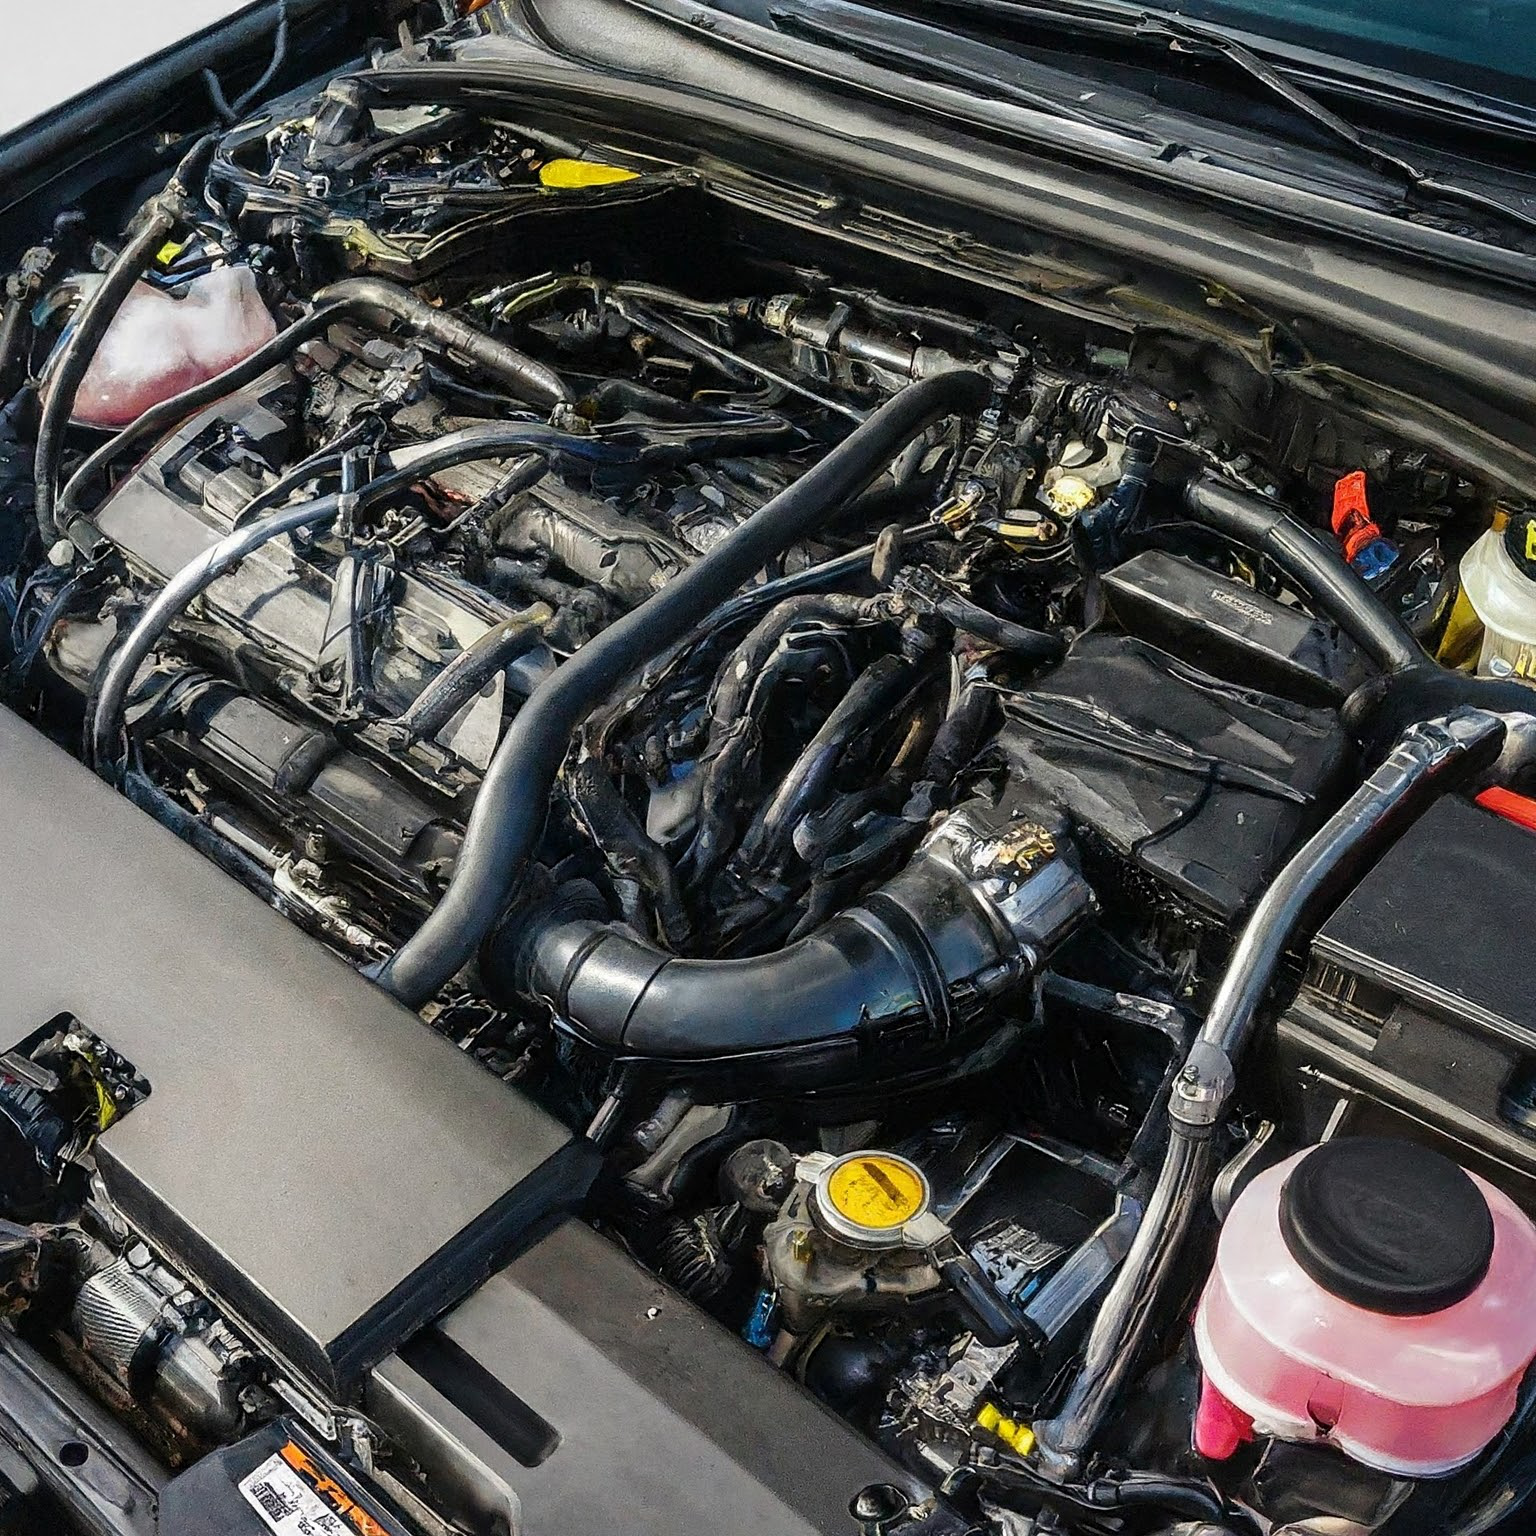
\includegraphics{images/engine.png}

}

\subcaption{\label{fig-r-1}R: Motor}

\end{minipage}%
%
\begin{minipage}{0.02\linewidth}
~\end{minipage}%
%
\begin{minipage}{0.49\linewidth}

\centering{

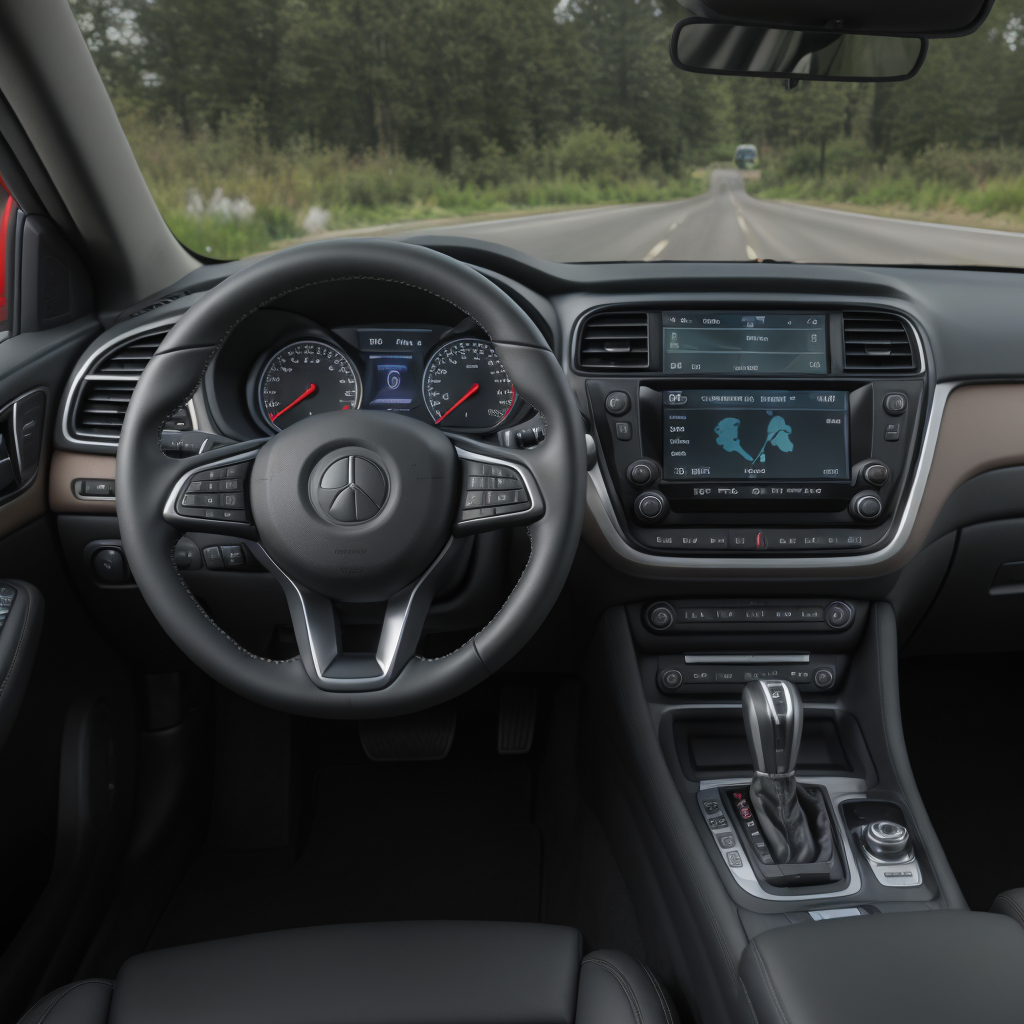
\includegraphics{images/dashboard.png}

}

\subcaption{\label{fig-rstudio-ide-1}RStudio IDE: Painel}

\end{minipage}%

\caption{\label{fig-r-vs-rstudio-ide-1}Analogia da diferença entre

\includegraphics[width=1.13em,height=1em]{getting_started_with_r_files/figure-pdf/fa-icon-9b00320707d42527dde67262afb33ded.pdf}
e RStudio}

\end{figure}%

\section{Como baixar e instalar o R}\label{como-baixar-e-instalar-o-r}

Para obter uma cópia e a versão oficial mais recente do

\includegraphics[width=1.13em,height=1em]{getting_started_with_r_files/figure-pdf/fa-icon-9b00320707d42527dde67262afb33ded.pdf},
acesse \href{https://cran.r-project.org/}{The Comprehensive R Archive
Network (CRAN)}. O

\includegraphics[width=1.13em,height=1em]{getting_started_with_r_files/figure-pdf/fa-icon-9b00320707d42527dde67262afb33ded.pdf}
é desenvolvido para as famílias de sistemas operacionais Unix, Windows e
Mac. Na CRAN, você encontrará 3 links para baixar o

\includegraphics[width=1.13em,height=1em]{getting_started_with_r_files/figure-pdf/fa-icon-9b00320707d42527dde67262afb33ded.pdf}
para Linux, macOS ou Windows:

\begin{itemize}
\item
  
\includegraphics[width=0.88em,height=1em]{getting_started_with_r_files/figure-pdf/fa-icon-8b189a97593caea540dafe6d05793999.pdf}:
  Clique em \textbf{Download R for Linux}, escolha sua distribuição e
  siga as instruções de instalação específicas para sua distribuição.
\item
  
\includegraphics[width=0.75em,height=1em]{getting_started_with_r_files/figure-pdf/fa-icon-934d7ce2d324ea402ee93b61438edad5.pdf}:
  Clique em \textbf{Download R for macOS}. Selecione o instalador que
  corresponda à sua versão do macOS, abra-o e siga as instruções na
  tela.
\item
  
\includegraphics[width=0.88em,height=1em]{getting_started_with_r_files/figure-pdf/fa-icon-b8a547d429c8db6a447f95260c20adaf.pdf}:
  Clique em \textbf{Download R for Windows} e, em seguida, clique em
  \textbf{base}. Depois, clique no primeiro link no topo da nova página
  e execute o instalador. O instalador irá guiá-lo através do processo
  de instalação.
\end{itemize}

\section{Como baixar e instalar o RStudio
IDE}\label{como-baixar-e-instalar-o-rstudio-ide}

Para obter a versão oficial mais recente do RStudio IDE, acesse
\url{https://posit.co/download/rstudio-desktop/}. Role a página para
baixo, selecione seu sistema operacional e baixe o instalador
apropriado. Abra o instalador e siga as instruções fornecidas.

Agora que você instalou o

\includegraphics[width=1.13em,height=1em]{getting_started_with_r_files/figure-pdf/fa-icon-9b00320707d42527dde67262afb33ded.pdf}
e o RStudio IDE, você está pronto para começar a trabalhar no RStudio
IDE. Assim como você interage principalmente com o volante e o painel de
um carro em vez do motor, você focará em usar a interface do RStudio IDE
para trabalhar com o

\includegraphics[width=1.13em,height=1em]{getting_started_with_r_files/figure-pdf/fa-icon-9b00320707d42527dde67262afb33ded.pdf}.

Ao abrir o RStudio IDE, você pode criar um novo script

\includegraphics[width=1.13em,height=1em]{getting_started_with_r_files/figure-pdf/fa-icon-9b00320707d42527dde67262afb33ded.pdf}
selecionando \textbf{File \textgreater{} New File \textgreater{} R
Script} ou usando o atalho de teclado \textbf{Ctrl + Shift + N}. Você
verá quatro painéis principais na interface, como mostrado na
Figura~\ref{fig-rstudio-ide-panels}:

\begin{itemize}
\tightlist
\item
  \textbf{Painel 1}: É onde você escreve, edita e salva seu código R.
\item
  \textbf{Painel 2}: Aqui você pode digitar os comandos do R e ver os
  resultados.
\item
  \textbf{Painel 3}: Este painel mostra os objetos do R (como variáveis
  ou dados) que você criou durante a sessão atual.
\item
  \textbf{Painel 4}: Vários elementos de saída, incluindo arquivos,
  gráficos e documentos de ajuda, são exibidos aqui.
\end{itemize}

\begin{figure}

\centering{

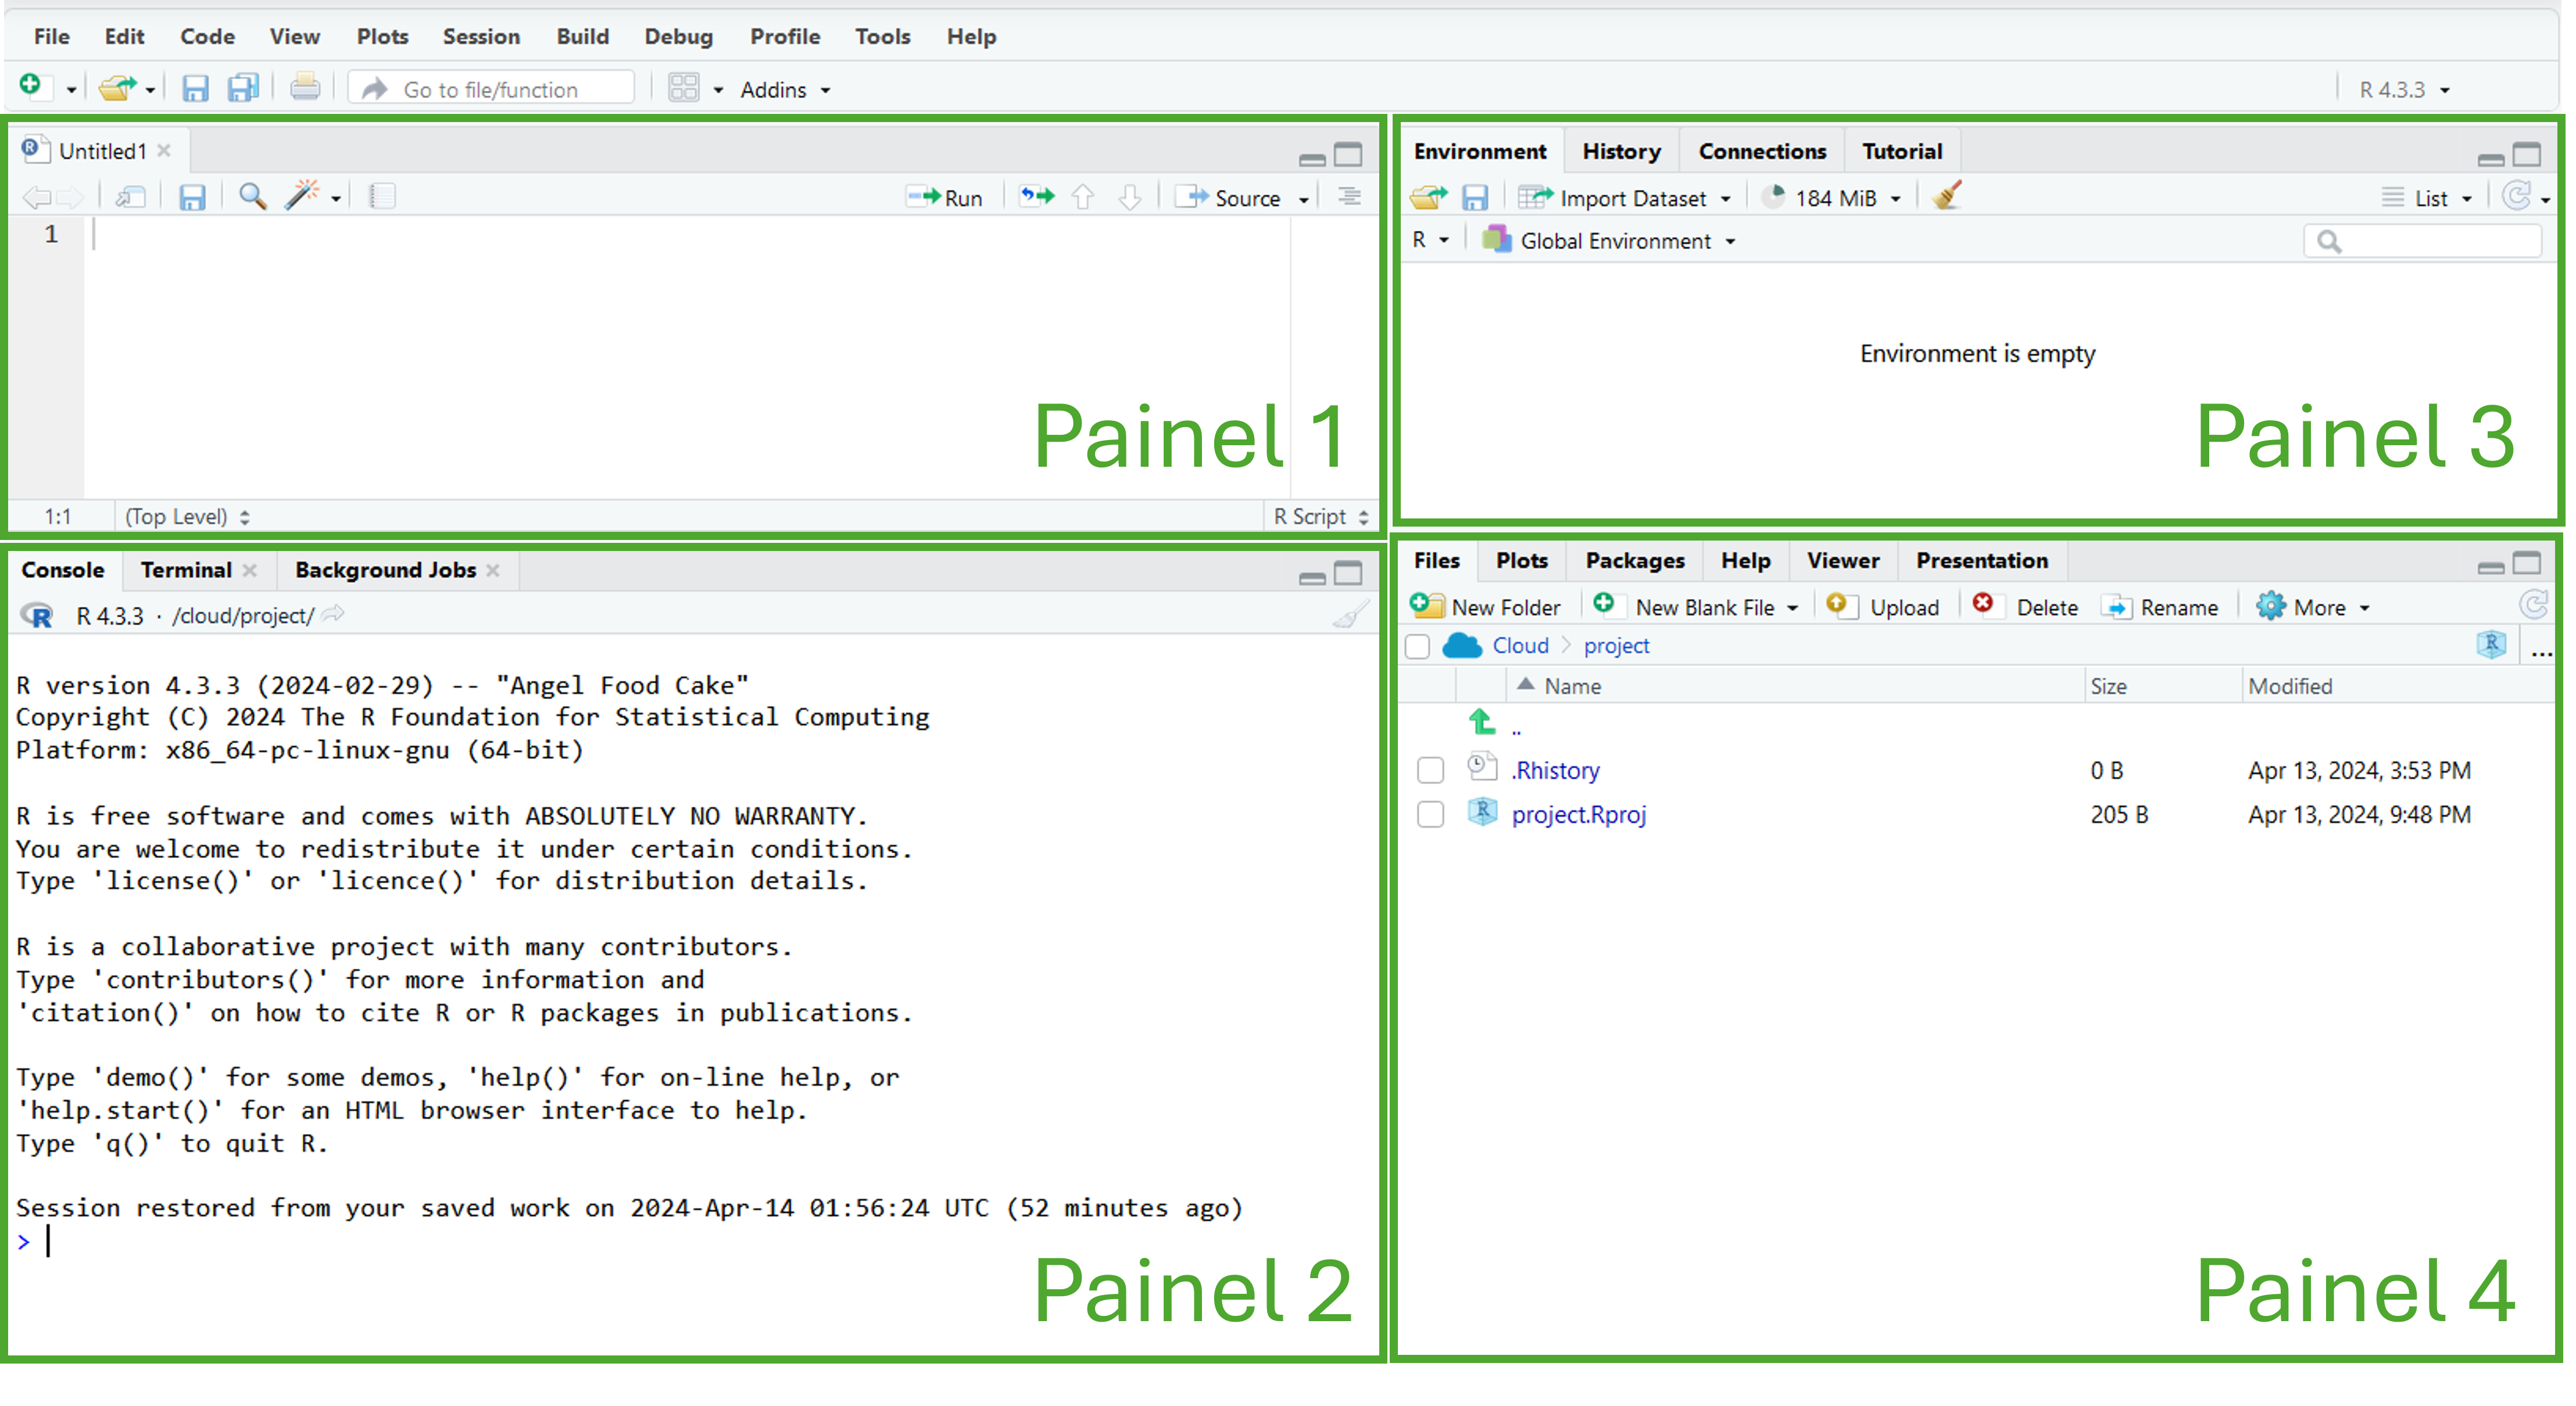
\includegraphics{images/panels_rstudio_ide.png}

}

\caption{\label{fig-rstudio-ide-panels}Painéis do RStudio IDE}

\end{figure}%

\subsection{Configurar e personalizar o RStudio
IDE}\label{configurar-e-personalizar-o-rstudio-ide}

Para personalizar seu espaço de trabalho, acesse \textbf{Tools
\textgreater{} Global Options}. Em seguida:

\begin{itemize}
\tightlist
\item
  Sempre inicie o
  
\includegraphics[width=1.13em,height=1em]{getting_started_with_r_files/figure-pdf/fa-icon-9b00320707d42527dde67262afb33ded.pdf}
  com uma sessão em branco, Figura~\ref{fig-r-blank-slate}:
\end{itemize}

\begin{figure}

\centering{

\captionsetup{labelsep=none}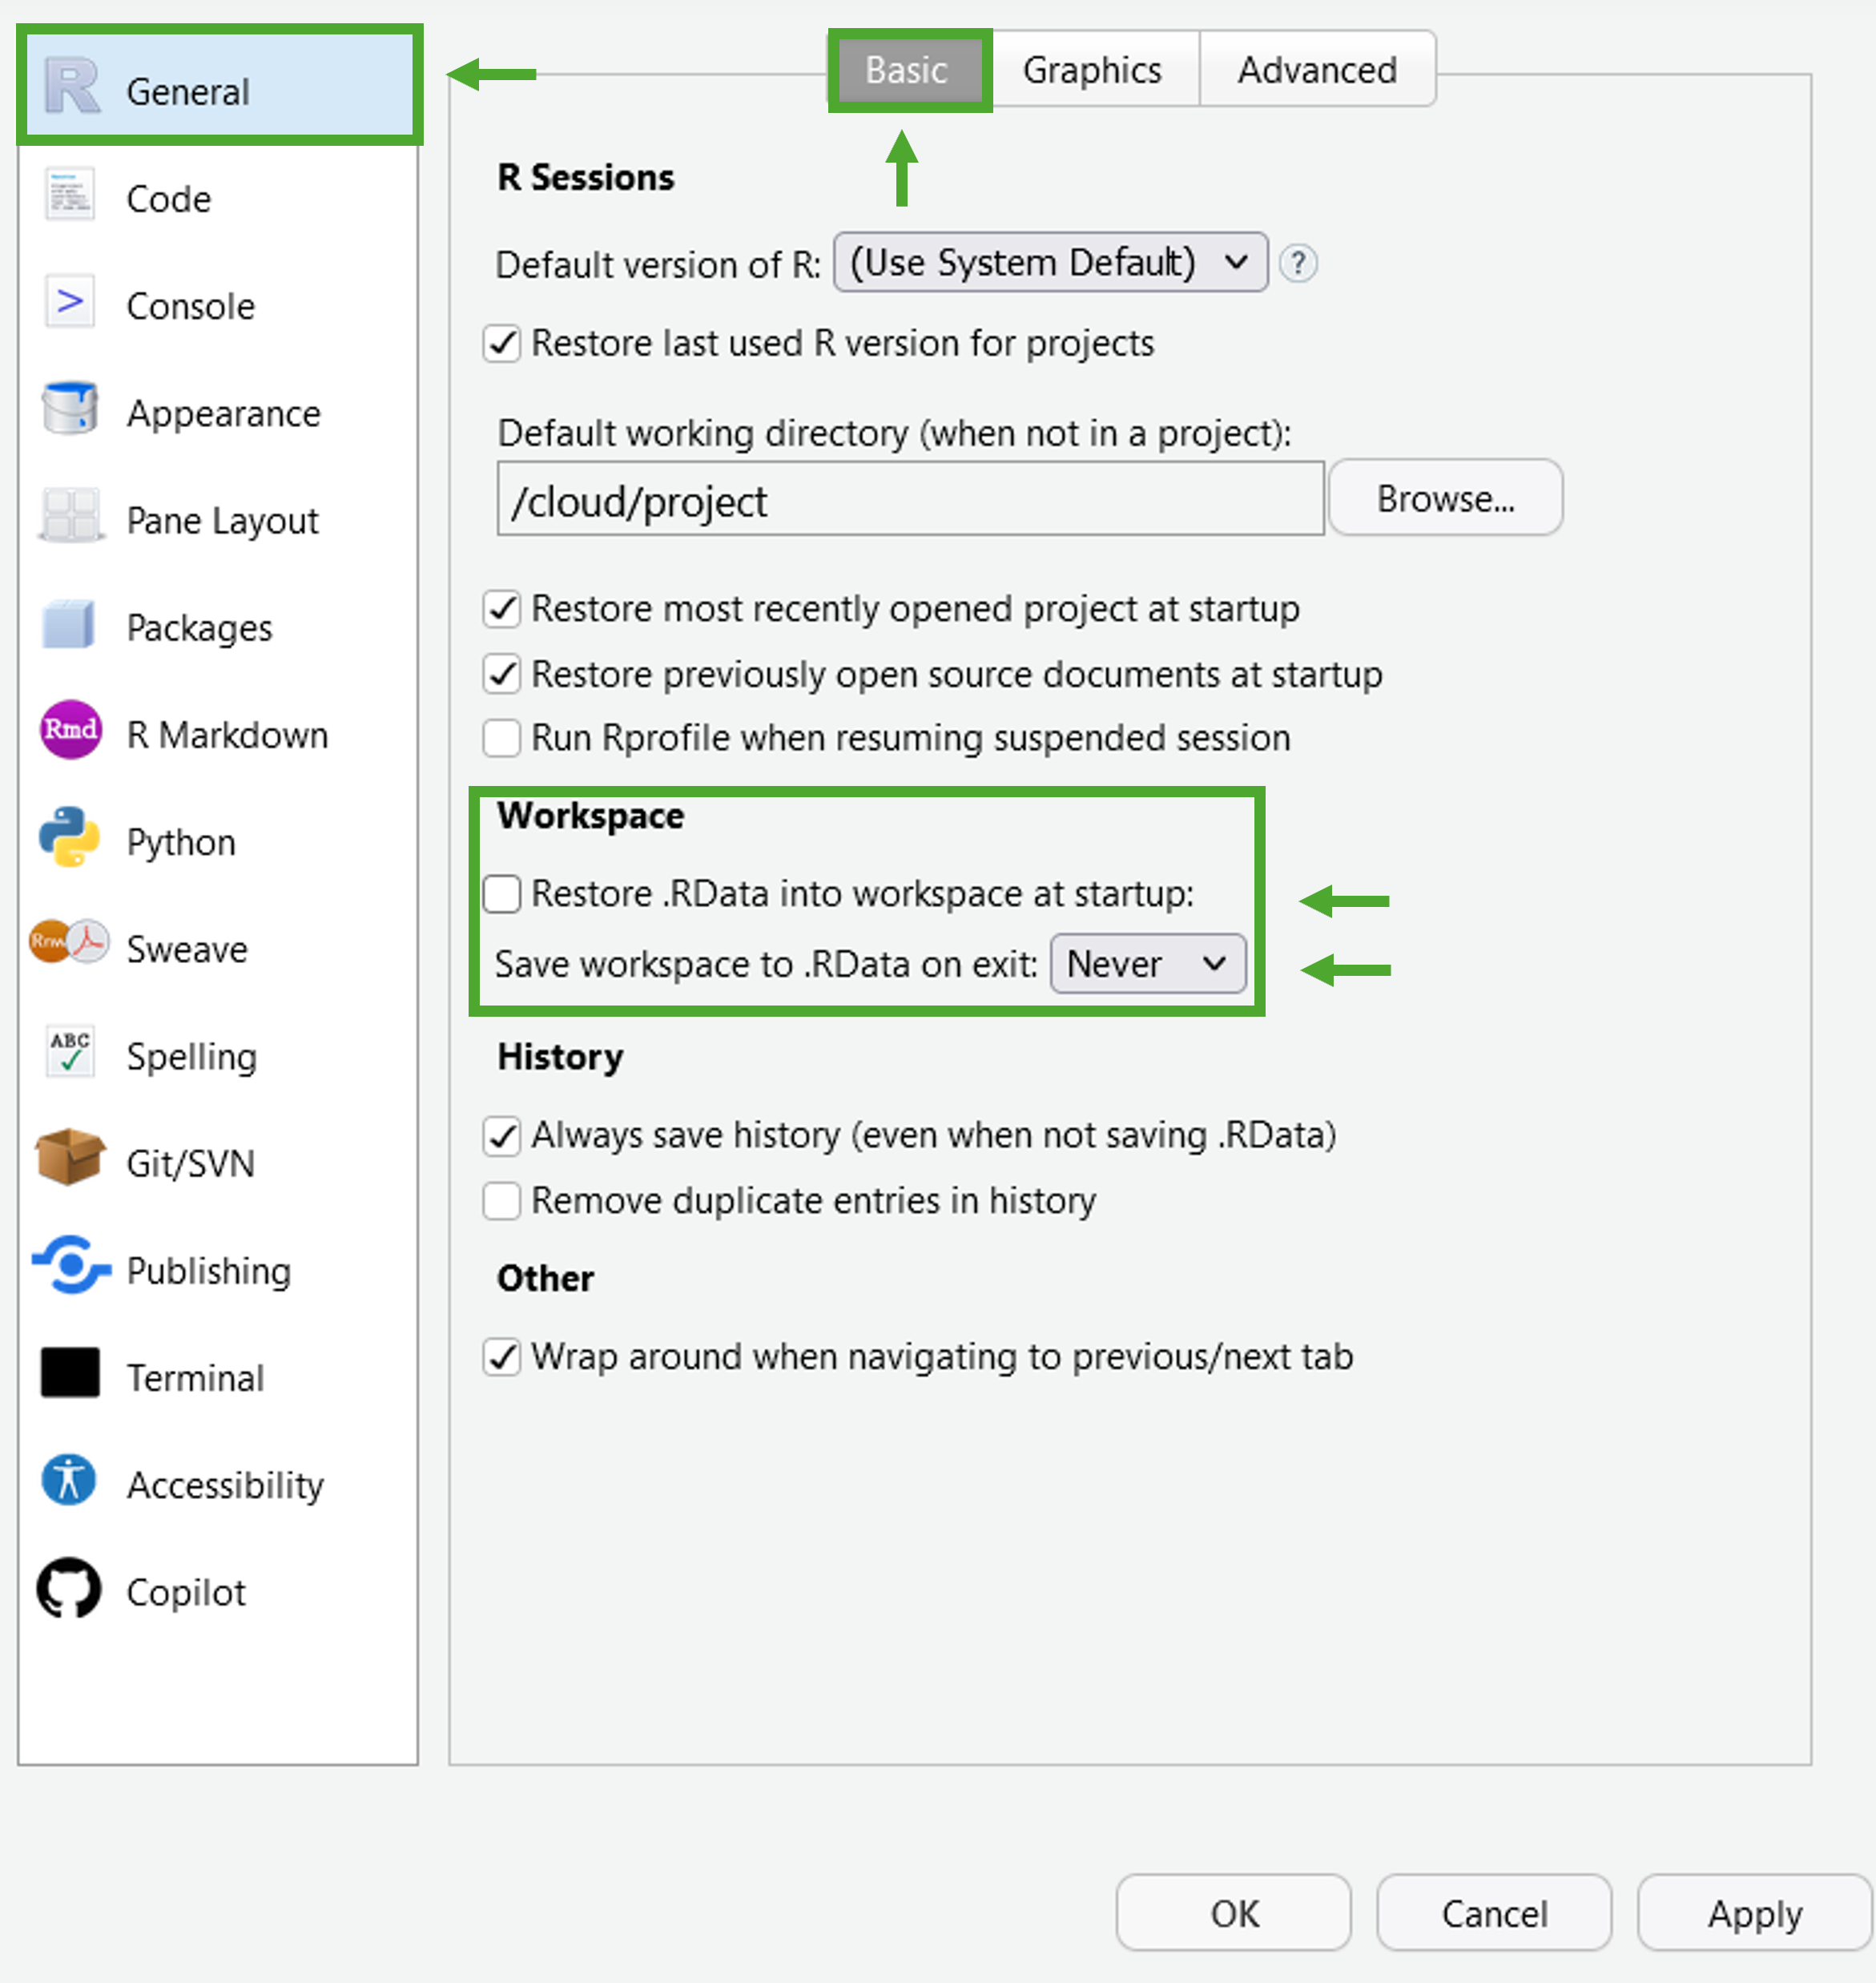
\includegraphics{images/r_blank slate.png}

}

\caption{\label{fig-r-blank-slate}}

\end{figure}%

\begin{itemize}
\tightlist
\item
  Use o operador de pipe nativo, \texttt{\textbar{}\textgreater{}},
  Figura~\ref{fig-native-pipe-operator}:
\end{itemize}

\begin{figure}

\centering{

\captionsetup{labelsep=none}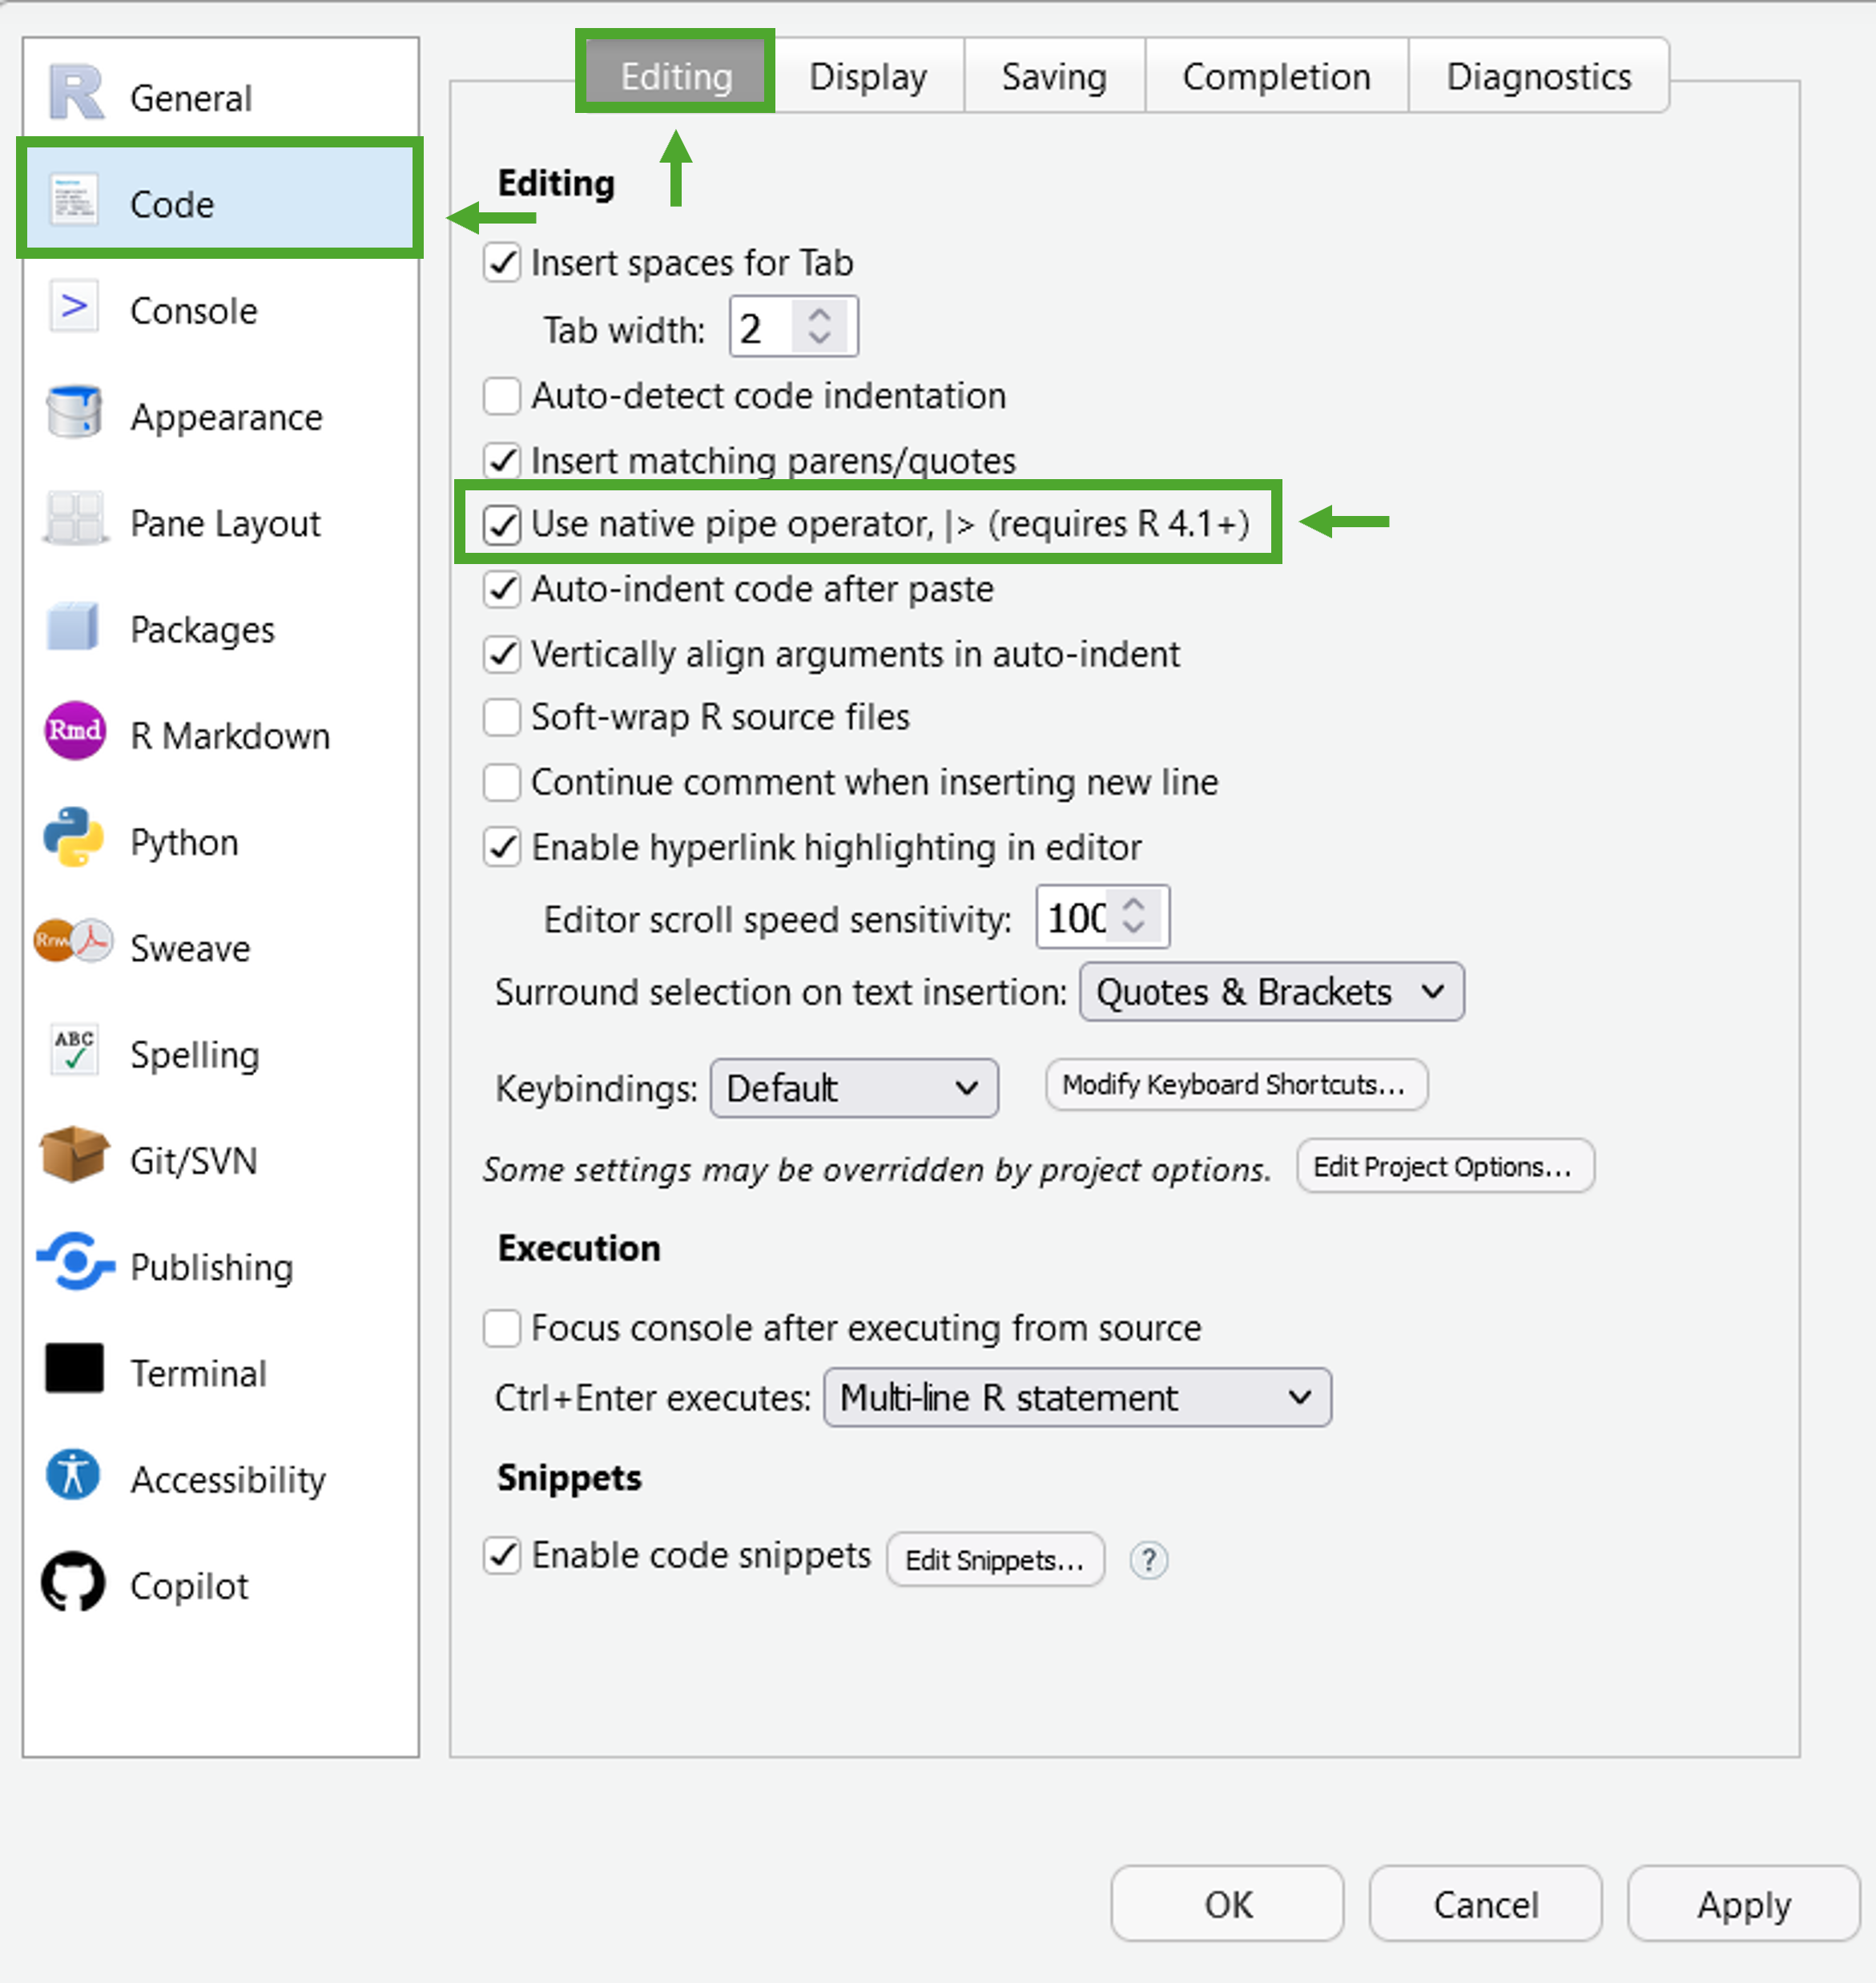
\includegraphics{images/native_pipe_operator.png}

}

\caption{\label{fig-native-pipe-operator}}

\end{figure}%

\begin{itemize}
\tightlist
\item
  Ajuste o tamanho da fonte e selecione um tema escuro,
  Figura~\ref{fig-font-size-dark-theme}:
\end{itemize}

\begin{figure}

\centering{

\captionsetup{labelsep=none}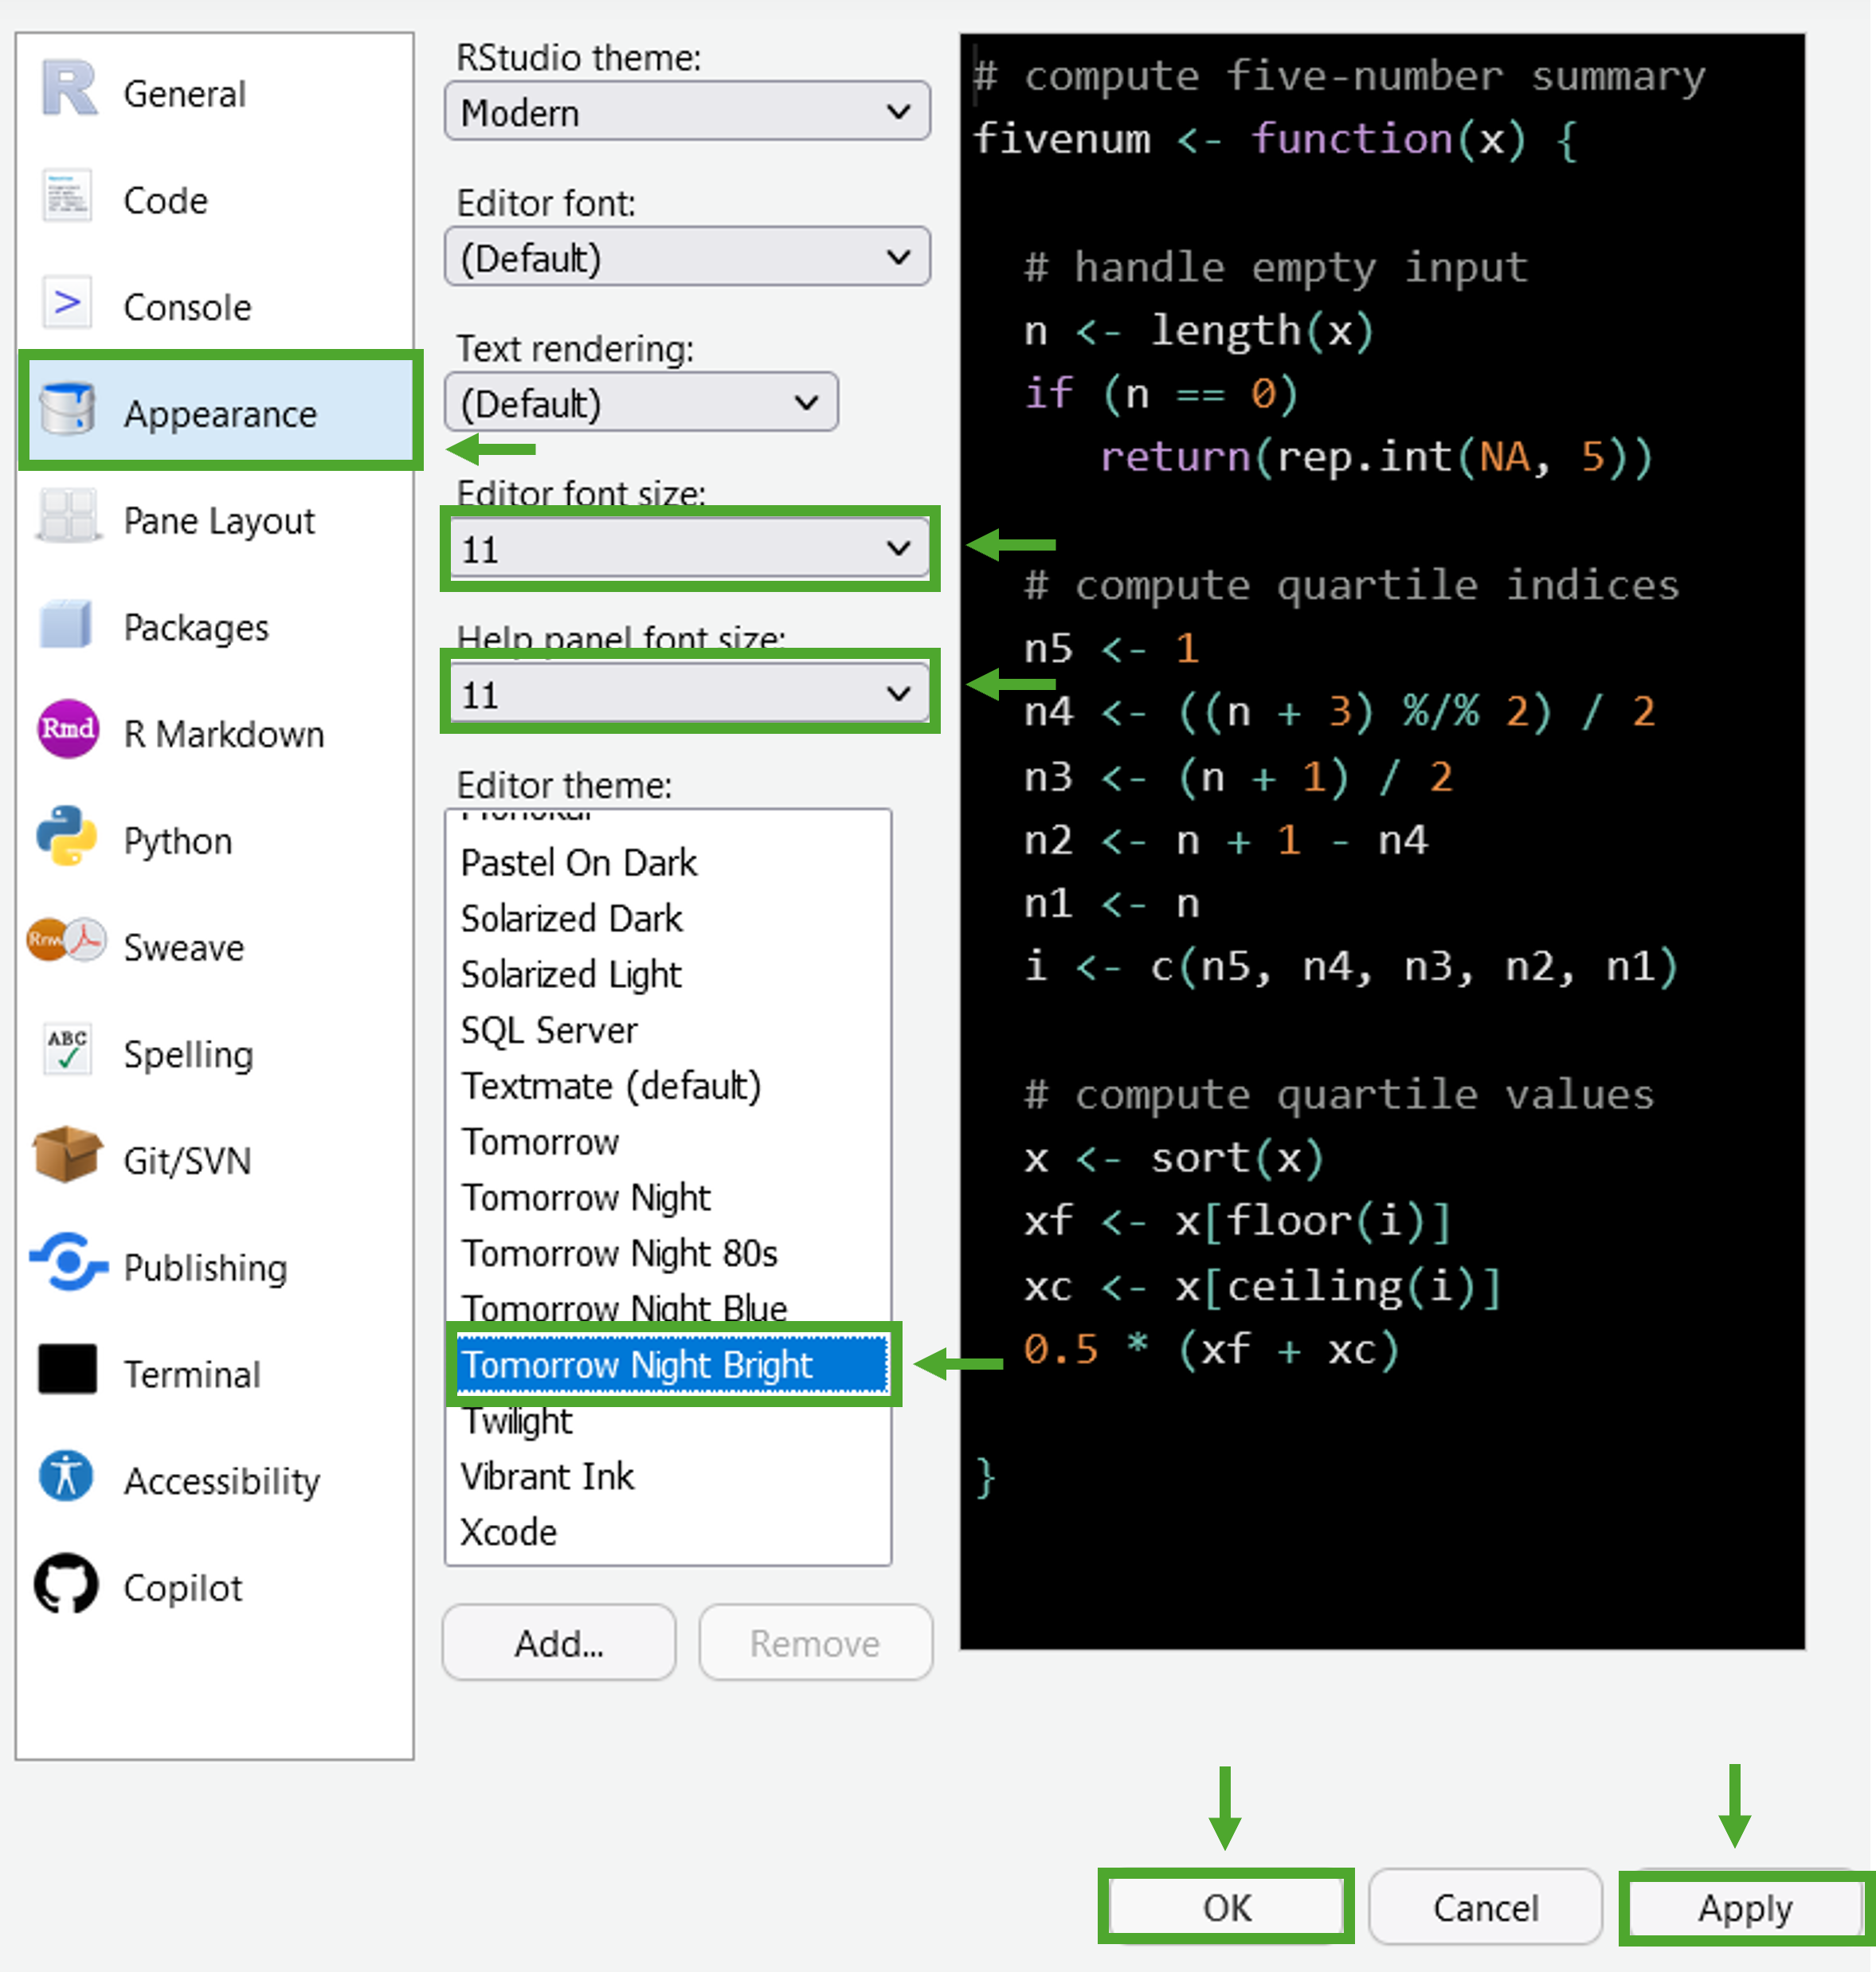
\includegraphics{images/font_size_dark_theme.png}

}

\caption{\label{fig-font-size-dark-theme}}

\end{figure}%

A aplicação dessas mudanças personalizará sua experiência com o RStudio
IDE, como mostrado na Figura~\ref{fig-customize-rstudio-ide}.

\begin{figure}

\centering{

\captionsetup{labelsep=none}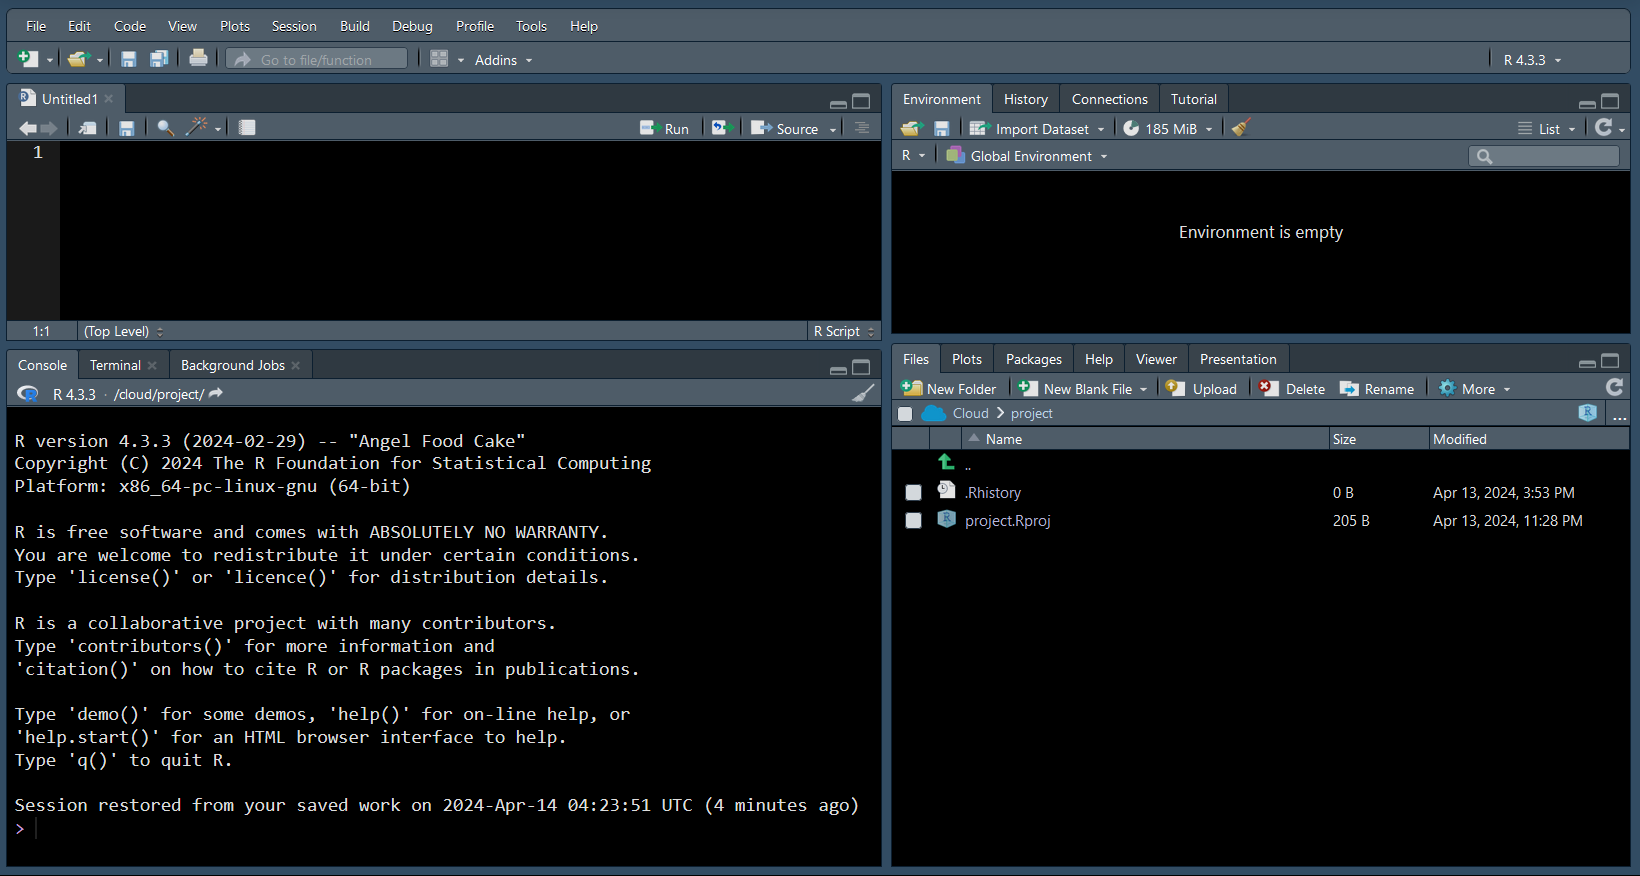
\includegraphics{images/customize_rstudio_ide.png}

}

\caption{\label{fig-customize-rstudio-ide}}

\end{figure}%

\chapter{Teoria ingênua dos
conjuntos}\label{teoria-inguxeanua-dos-conjuntos}

A teoria dos conjuntos é um ramo da matemática que estuda coleções
denominadas conjuntos. Compreender a teoria dos conjuntos é fundamental,
pois ela serve como base para a teoria da probabilidade, que por sua vez
é crucial para o estudo da estatística. No entanto, um conhecimento
básico da teoria dos conjuntos é suficiente para entender os princípios
fundamentais da probabilidade e da estatística, sem a necessidade de um
formalismo excessivo \footnote{Para uma apresentação detalhada e clara
  da teoria dos conjuntos usando um sistema de axiomas, você pode
  consultar (\citeproc{ref-halmos_teoria_2001}{Halmos 2001})}.

\section{Conjuntos}\label{conjuntos}

\begin{definition}[Conjunto]\protect\hypertarget{def-set}{}\label{def-set}

Um \textbf{conjunto} é uma coleção não ordenada de elementos únicos, ou
pode ser uma coleção vazia, sem nenhum elemento.

\end{definition}

Podemos denotar um conjunto usando uma letra arbitrária como \(A\) e
descrevê-lo listando seus elementos entre chaves. Por exemplo,
\(A = \{ 1,2 \}\) é o conjunto cujos elementos são os números \(1\) e
\(2\). Com base em Definição~\ref{def-set} e na notação anterior, é
importante fazer as seguintes observações:

\begin{itemize}
\item
  \(A = \{ 1, 2 \}\) e \(B = \{ 2, 1 \}\) são o mesmo conjunto porque
  conjuntos são coleções não ordenadas onde a ordem não é definida.
\item
  \(C = \{ 1, 1, 2, 2 \}\) não está bem definido porque um conjunto
  contém elementos únicos, onde a especificação correta seria
  \(C = \{ 1, 2 \}\).
\item
  Existe um conjunto, denotado por \(\emptyset = \{ \}\), chamado
  \textbf{conjunto vazio}, que não possui elementos.
\item
  É possível que os elementos de um conjunto sejam eles próprios
  conjuntos. Por exemplo, \(D = \{ \{ 1, 2\}, 3 \}\) é um conjunto que
  contém o conjunto \(\{ 1, 2\}\) e o número \(3\)
\end{itemize}

O pacote \texttt{sets} do

\includegraphics[width=1.13em,height=1em]{naive_set_theory_files/figure-pdf/fa-icon-9b00320707d42527dde67262afb33ded.pdf}
pode ser usado para ilustrar as ideias mencionadas acima para entender o
conceito de conjunto. Primeiramente, podemos criar dois conjuntos e
verificar se os dois conjuntos são iguais:

\begin{Shaded}
\begin{Highlighting}[]
\FunctionTok{library}\NormalTok{(sets)}
\NormalTok{A }\OtherTok{\textless{}{-}} \FunctionTok{set}\NormalTok{(}\DecValTok{1}\NormalTok{, }\DecValTok{2}\NormalTok{)}
\NormalTok{A}
\CommentTok{\#\textgreater{} \{1, 2\}}
\NormalTok{B }\OtherTok{\textless{}{-}} \FunctionTok{set}\NormalTok{(}\DecValTok{2}\NormalTok{, }\DecValTok{1}\NormalTok{)}
\NormalTok{B}
\CommentTok{\#\textgreater{} \{1, 2\}}
\NormalTok{A }\SpecialCharTok{==}\NormalTok{ B}
\CommentTok{\#\textgreater{} [1] TRUE}
\end{Highlighting}
\end{Shaded}

Também podemos verificar a propriedade de elementos únicos em um
conjunto:

\begin{Shaded}
\begin{Highlighting}[]
\NormalTok{C }\OtherTok{\textless{}{-}} \FunctionTok{set}\NormalTok{(}\DecValTok{1}\NormalTok{, }\DecValTok{1}\NormalTok{, }\DecValTok{2}\NormalTok{, }\DecValTok{2}\NormalTok{)}
\NormalTok{C}
\CommentTok{\#\textgreater{} \{1, 2\}}
\end{Highlighting}
\end{Shaded}

Além disso, podemos criar um conjunto vazio:

\begin{Shaded}
\begin{Highlighting}[]
\NormalTok{vazio }\OtherTok{\textless{}{-}} \FunctionTok{set}\NormalTok{()}
\NormalTok{vazio}
\CommentTok{\#\textgreater{} \{\}}
\end{Highlighting}
\end{Shaded}

Por último, podemos definir um conjunto cujos elementos podem ser
conjuntos:

\begin{Shaded}
\begin{Highlighting}[]
\NormalTok{D }\OtherTok{\textless{}{-}} \FunctionTok{set}\NormalTok{(A, }\DecValTok{3}\NormalTok{)}
\NormalTok{D}
\CommentTok{\#\textgreater{} \{3, \{1, 2\}\}}
\end{Highlighting}
\end{Shaded}

\begin{definition}[Relação de
pertença]\protect\hypertarget{def-membership-relation}{}\label{def-membership-relation}

Se \(a\) é um elemento de \(A\), expressamos essa condição como
\(a \in A\). Caso contrário, expressamos que \(a\) não é um elemento de
\(A\) com \(a \notin A\). Na teoria dos conjuntos, \(\in\) é conhecido
como a relação \emph{``é um elemento de''}.

\end{definition}

Por exemplo, se \(A = \{ 1 , 2 \}\) então \(1 \in A\) e \(3 \notin A\).
Em

\includegraphics[width=1.13em,height=1em]{naive_set_theory_files/figure-pdf/fa-icon-9b00320707d42527dde67262afb33ded.pdf},
podemos verificar se um elemento pertence a um conjunto usando o
operador \texttt{\%e\%} do pacote \texttt{sets}, que representa a
relação \(\in\):

\begin{Shaded}
\begin{Highlighting}[]
\DecValTok{1} \SpecialCharTok{\%e\%}\NormalTok{ A}
\CommentTok{\#\textgreater{} [1] TRUE}
\DecValTok{3} \SpecialCharTok{\%e\%}\NormalTok{ A}
\CommentTok{\#\textgreater{} [1] FALSE}
\end{Highlighting}
\end{Shaded}

Às vezes, não é possível listar os elementos de um conjunto porque os
elementos são infinitos ou porque não sabemos exatamente quais são. No
entanto, se sabemos a propriedade que cada elemento deve ter, podemos
usar uma notação matemática conhecida como \textbf{notação construtor de
conjuntos} para descrever o conjunto. Essa notação é especificada como
\(\{ x \in \Omega: P(x) \}\), onde \(x\) é um elemento genérico que
pertence a \(\Omega\) com a propriedade \(P(x)\). \(\Omega\)\footnote{\(\Omega\)
  é chamado Ômega} é conhecido como \textbf{universo de discurso} e se
refere ao conjunto que contém todos os elementos em consideração a
partir dos quais o valor de \(x\) pode ser escolhido. Por exemplo:

\begin{itemize}
\tightlist
\item
  \(E = \{ x \in \Omega: x \text{ é um cachorro} \}\) onde \(E\) é o
  conjunto que contém todos os \(x\) que são cachorros. Nesse caso,
  \(P(x)\) refere-se a ter a propriedade de ser um cachorro e \(\Omega\)
  pode ser o conjunto dos seres vivos.
\item
  \(F = \{ x \in \mathbb{N} : x > 5 \}\) onde \(F\) contém todos os
  números maiores que \(5\) que são números naturais. Nesse caso,
  \(P(x)\) refere-se a todos os \(x\) maiores que \(5\) e \(\Omega\) é o
  conjunto dos números naturais.
\end{itemize}

Infelizmente, o

\includegraphics[width=1.13em,height=1em]{naive_set_theory_files/figure-pdf/fa-icon-9b00320707d42527dde67262afb33ded.pdf}
só pode manipular objetos que podem ser representados como números e que
são finitos. Portanto, o uso de pacotes como \texttt{sets} não permite
representar conjuntos como \(E\) ou \(F\) no

\includegraphics[width=1.13em,height=1em]{naive_set_theory_files/figure-pdf/fa-icon-9b00320707d42527dde67262afb33ded.pdf}.

\begin{definition}[Subconjunto]\protect\hypertarget{def-subset}{}\label{def-subset}

Um conjunto \(A\) é um \textbf{subconjunto} de um conjunto \(B\) se
todos os elementos de \(A\) também sejam elementos de \(B\). Essa
condição pode ser expressa através da notação \(A \subseteq B\). Por
outro lado, se existir um elemento que pertença a \(A\), mas não
pertença a \(B\), representamos essa situação como \(A \nsubseteq B\).
Na teoria dos conjuntos, \(\subseteq\) é conhecido como a relação de
\emph{``inclusão''}.

\end{definition}

A Figura~\ref{fig-subset-venn-diagram} ilustra a
Definição~\ref{def-subset} usando um \textbf{diagrama de
Venn}\footnote{Um diagrama de Venn é uma ferramenta visual que utiliza
  formas fechadas para representar conjuntos e ilustrar como seus
  elementos se relacionam.}.

\begin{figure}

\centering{

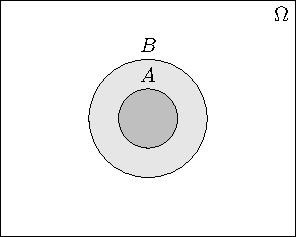
\includegraphics[width=0.5\textwidth,height=\textheight]{naive_set_theory_files/figure-pdf/fig-subset-venn-diagram-1.pdf}

}

\caption{\label{fig-subset-venn-diagram}\(A \subseteq B\) representado
por um diagrama de Venn onde \(\Omega\) é o universo de discurso}

\end{figure}%

Por exemplo, se \(A = \{ 1 , 2 \}\) e \(G = \{ 1, 2, 3\}\) então
\(A \subseteq G\) porque \(1 \in A\), \(1 \in G\), \(2 \in A\) e
\(2 \in G\). No entanto, \(G \nsubseteq A\) porque \(3 \in G\) e
\(3 \notin A\). Em

\includegraphics[width=1.13em,height=1em]{naive_set_theory_files/figure-pdf/fa-icon-9b00320707d42527dde67262afb33ded.pdf},
podemos verificar se um conjunto é um subconjunto de um conjunto usando
o operador \texttt{\textless{}=} do pacote \texttt{sets}, que representa
a relação \(\subseteq\):

\begin{Shaded}
\begin{Highlighting}[]
\NormalTok{G }\OtherTok{\textless{}{-}} \FunctionTok{set}\NormalTok{(}\DecValTok{1}\NormalTok{, }\DecValTok{2}\NormalTok{, }\DecValTok{3}\NormalTok{)}
\NormalTok{G}
\CommentTok{\#\textgreater{} \{1, 2, 3\}}
\NormalTok{A }\SpecialCharTok{\textless{}=}\NormalTok{ G}
\CommentTok{\#\textgreater{} [1] TRUE}
\NormalTok{G }\SpecialCharTok{\textless{}=}\NormalTok{ A}
\CommentTok{\#\textgreater{} [1] FALSE}
\end{Highlighting}
\end{Shaded}

\begin{definition}[Igualdade de
conjuntos]\protect\hypertarget{def-set-equality}{}\label{def-set-equality}

Com base em Definição~\ref{def-subset} podemos estabelecer uma definição
equivalente para a igualdade de conjuntos. Dois conjuntos, \(A\) e
\(B\), são considerados iguais, \(A = B\), se e somente se
\(A \subseteq B\) e \(B \subseteq A\). Em outras palavras, ambos os
conjuntos devem conter exatamente os mesmos elementos para serem
considerados iguais.

\end{definition}

\section{Operações com conjuntos}\label{operauxe7uxf5es-com-conjuntos}

\begin{definition}[União de
conjuntos]\protect\hypertarget{def-union}{}\label{def-union}

A união de dois conjuntos \(A\) e \(B\), denotada por \(A \cup B\), é o
conjunto de todos os elementos que estão em \(A\) \textbf{ou} em \(B\).
\(A \cup B\) também é um conjunto e pode ser definido usando notação
construtor de conjuntos como
\(A \cup B = \{x \in \Omega : x \in A \textbf{ ou } x \in B \}\)

\end{definition}

A Figura~\ref{fig-union-venn-diagram} ilustra a
Definição~\ref{def-union} usando um diagrama de Venn.

\begin{figure}

\centering{

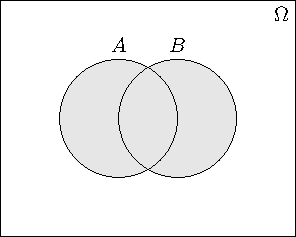
\includegraphics[width=0.5\textwidth,height=\textheight]{naive_set_theory_files/figure-pdf/fig-union-venn-diagram-1.pdf}

}

\caption{\label{fig-union-venn-diagram}\(A \cup B\) representado por um
diagrama de Venn onde \(\Omega\) é o universo de discurso}

\end{figure}%

Por exemplo, se \(A = \{ 1, 2 \}\) e \(H = \{ 2, 3 \}\), então
\(A \cup H = \{ 1, 2, 3 \}\). Em

\includegraphics[width=1.13em,height=1em]{naive_set_theory_files/figure-pdf/fa-icon-9b00320707d42527dde67262afb33ded.pdf},
utilizando o pacote \texttt{sets}, o operador \texttt{\textbar{}} é
utilizado para representar a união, \(\cup\), de dois conjuntos da
seguinte maneira:

\begin{Shaded}
\begin{Highlighting}[]
\NormalTok{H }\OtherTok{\textless{}{-}} \FunctionTok{set}\NormalTok{(}\DecValTok{2}\NormalTok{, }\DecValTok{3}\NormalTok{)}
\NormalTok{A }\SpecialCharTok{|}\NormalTok{ H}
\CommentTok{\#\textgreater{} \{1, 2, 3\}}
\end{Highlighting}
\end{Shaded}

\begin{definition}[Interseção de
conjuntos]\protect\hypertarget{def-intersection}{}\label{def-intersection}

A interseção de dois conjuntos \(A\) e \(B\), denotada por \(A \cap B\),
é o conjunto de todos os elementos que estão em \(A\) \textbf{e} em
\(B\). \(A \cap B\) também é um conjunto e pode ser definido usando
notação construtor de conjuntos como
\(A \cap B = \{ x \in \Omega : x \in A \textbf{ e } x \in B \}\).

\end{definition}

A Figura~\ref{fig-intersection-venn-diagram} ilustra a
Definição~\ref{def-intersection} usando um diagrama de Venn.

\begin{figure}

\centering{

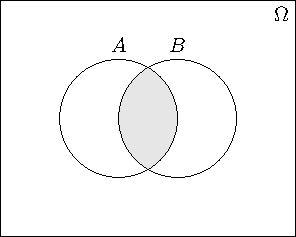
\includegraphics[width=0.5\textwidth,height=\textheight]{naive_set_theory_files/figure-pdf/fig-intersection-venn-diagram-1.pdf}

}

\caption{\label{fig-intersection-venn-diagram}\(A \cap B\) representado
por um diagrama de Venn onde \(\Omega\) é o universo de discurso}

\end{figure}%

Por exemplo, se \(A = \{ 1, 2 \}\) e \(H = \{ 2, 3 \}\), então
\(A \cap H = \{ 2 \}\). Em

\includegraphics[width=1.13em,height=1em]{naive_set_theory_files/figure-pdf/fa-icon-9b00320707d42527dde67262afb33ded.pdf},
utilizando o pacote \texttt{sets}, o operador \texttt{\&} é utilizado
para representar a interseção, \(\cap\), de dois conjuntos da seguinte
maneira:

\begin{Shaded}
\begin{Highlighting}[]
\NormalTok{A }\SpecialCharTok{\&}\NormalTok{ H}
\CommentTok{\#\textgreater{} \{2\}}
\end{Highlighting}
\end{Shaded}

\begin{definition}[Diferença de
conjuntos]\protect\hypertarget{def-difference}{}\label{def-difference}

A diferença de dois conjuntos \(A\) e \(B\), denotada por
\(A \setminus B\), é o conjunto de todos os elementos que pertencem a
\(A\), mas não a \(B\). \(A \setminus B\) também é um conjunto e pode
ser definido usando notação construtor de conjuntos como
\(A \setminus B = \{ x \in \Omega : x \in A \text{ e } x \notin B \}\).

\end{definition}

A Figura~\ref{fig-difference-venn-diagram} ilustra a
Definição~\ref{def-difference} usando um diagrama de Venn.

\begin{figure}

\centering{

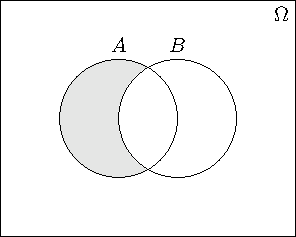
\includegraphics[width=0.5\textwidth,height=\textheight]{naive_set_theory_files/figure-pdf/fig-difference-venn-diagram-1.pdf}

}

\caption{\label{fig-difference-venn-diagram}\(A \setminus B\)
representado por um diagrama de Venn onde \(\Omega\) é o universo de
discurso}

\end{figure}%

Por exemplo, se \(A = \{ 1, 2 \}\) e \(H = \{ 2, 3 \}\), então
\(A \setminus H = \{ 1 \}\) e \(H \setminus A = \{ 3 \}\). Em

\includegraphics[width=1.13em,height=1em]{naive_set_theory_files/figure-pdf/fa-icon-9b00320707d42527dde67262afb33ded.pdf},
utilizando o pacote \texttt{sets}, o operador \texttt{-} é utilizado
para representar a diferença, \(\setminus\), de dois conjuntos da
seguinte maneira:

\begin{Shaded}
\begin{Highlighting}[]
\NormalTok{A }\SpecialCharTok{{-}}\NormalTok{ H}
\CommentTok{\#\textgreater{} \{1\}}
\NormalTok{H }\SpecialCharTok{{-}}\NormalTok{ A}
\CommentTok{\#\textgreater{} \{3\}}
\end{Highlighting}
\end{Shaded}

\begin{definition}[Complemento de um
conjunto]\protect\hypertarget{def-complement}{}\label{def-complement}

Se \(A\) e \(\Omega\) são conjuntos, onde e \(\Omega\) é o universo de
discurso, o complemento de \(A\), denotado por \(A^c\), é o conjunto
\(\Omega \setminus A\). Ou seja,
\(A^c = \{x \in \Omega: x \notin A \text{ e } A \subseteq \Omega \}\).

\end{definition}

A Figura~\ref{fig-complement-venn-diagram} ilustra a
Definição~\ref{def-complement} usando um diagrama de Venn.

\begin{figure}

\centering{

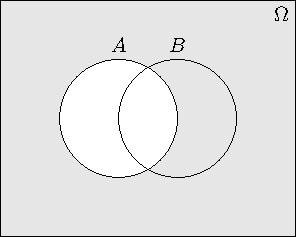
\includegraphics[width=0.5\textwidth,height=\textheight]{naive_set_theory_files/figure-pdf/fig-complement-venn-diagram-1.pdf}

}

\caption{\label{fig-complement-venn-diagram}\(A^c\) representado por um
diagrama de Venn onde \(\Omega\) é o universo de discurso}

\end{figure}%

Por exemplo, se \(A = \{ 1, 2 \}\) e \(\Omega = \{ 1, 2, 3, 4 \}\),
então \(A^c = \{ 3, 4 \}\). Em

\includegraphics[width=1.13em,height=1em]{naive_set_theory_files/figure-pdf/fa-icon-9b00320707d42527dde67262afb33ded.pdf},
utilizando o pacote \texttt{sets}, podemos determinar \(A^c\) da
seguinte maneira:

\begin{Shaded}
\begin{Highlighting}[]
\NormalTok{omega }\OtherTok{\textless{}{-}} \FunctionTok{set}\NormalTok{(}\DecValTok{1}\NormalTok{, }\DecValTok{2}\NormalTok{, }\DecValTok{3}\NormalTok{, }\DecValTok{4}\NormalTok{)}
\NormalTok{omega }\SpecialCharTok{{-}}\NormalTok{ A}
\CommentTok{\#\textgreater{} \{3, 4\}}
\end{Highlighting}
\end{Shaded}

\section{O conjunto vazio e o conjunto
potência}\label{o-conjunto-vazio-e-o-conjunto-potuxeancia}

O conjunto vazio, \(\emptyset\), tem certas características que podem
parecer contraintuitivas. Em primeiro lugar, só pode haver um conjunto
vazio porque quaisquer dois conjuntos que não contenham nenhum elemento
são idênticos. Conforme declarado na Definição~\ref{def-set-equality},
conjuntos são considerados iguais se eles têm os mesmos elementos. Como
ambos os conjuntos vazios não contêm elementos, eles são considerados o
mesmo conjunto.

Outra propriedade aparentemente contraintuitiva é que o conjunto vazio é
um subconjunto de todos os conjuntos. Se temos um conjunto \(A\), e
afirmamos que o conjunto vazio não é um subconjunto de \(A\), denotado
por \(\emptyset \subseteq A\), então, de acordo com a
Definição~\ref{def-subset}, deve existir um elemento que pertença a
\(\emptyset\), mas não a \(A\). No entanto, como o conjunto vazio não
tem nenhum elemento, é impossível que um elemento pertença a
\(\emptyset\). Portanto, a única maneira de evitar uma contradição é
aceitar que o conjunto vazio é um subconjunto de todos os conjuntos,
denotado por \(\emptyset \subseteq A\).

Podemos resumir os resultados acima da seguinte maneira:

\begin{theorem}[Unicidade do conjunto
vazio]\protect\hypertarget{thm-empty-set-uniqueness}{}\label{thm-empty-set-uniqueness}

Só existe um conjunto vazio. Em outras palavras, se \(\emptyset\) e
\(\emptyset^{'}\) são ambos conjuntos vazios, então \(\emptyset\) é
igual a \(\emptyset^{'}\), \(\emptyset = \emptyset^{'}\).

\end{theorem}

\begin{theorem}[Propriedade de subconjunto do conjunto
vazio]\protect\hypertarget{thm-empty-set-subset}{}\label{thm-empty-set-subset}

O conjunto vazio é um subconjunto de todos os conjuntos. Para qualquer
conjunto \(A\), o conjunto vazio, \(\emptyset\), é um subconjunto de
\(A\), \(\emptyset \subseteq A\).

\end{theorem}

Há também um conjunto chamado \textbf{conjunto das potências}. O
conjunto das potências de um conjunto \(A\), denotado como
\(\mathcal{P}(A)\), é um conjunto que contém todos os subconjuntos de
\(A\). Podemos defini-lo como:

\begin{definition}[Conjunto das
potências]\protect\hypertarget{def-power-set}{}\label{def-power-set}

Se \(A\) é um conjunto, então o conjunto que contém todos os
subconjuntos de \(A\), denotado como \(\mathcal{P}(A)\), é definido como
\(\mathcal{P}(A) = \{ B: B \subseteq A \}\).

\end{definition}

Por exemplo, se \(A = \{ 1, 2 \}\) então
\(\mathcal{P}(A) = \{ \emptyset, \{ 1 \}, \{ 2 \}, A \} = \{ \emptyset, \{ 1 \}, \{ 2 \}, \{ 1,2 \} \}\)
porque \(\emptyset \subseteq A\) pelo
Teorema~\ref{thm-empty-set-subset}, \(\{ 1 \} \subseteq A\),
\(\{ 2 \} \subseteq A\) e \(A = \{ 1, 2 \} \subseteq A\). Em

\includegraphics[width=1.13em,height=1em]{naive_set_theory_files/figure-pdf/fa-icon-9b00320707d42527dde67262afb33ded.pdf},
podemos construir o conjunto das potências de um conjunto \(A\),
\(\mathcal{P}(A)\), como \texttt{2\^{}A} utilizando o pacote
\texttt{sets} da seguinte maneira:

\begin{Shaded}
\begin{Highlighting}[]
\NormalTok{potencia\_A }\OtherTok{\textless{}{-}} \DecValTok{2}\SpecialCharTok{\^{}}\NormalTok{A}
\NormalTok{potencia\_A}
\CommentTok{\#\textgreater{} \{\{\}, \{1\}, \{2\}, \{1, 2\}\}}
\end{Highlighting}
\end{Shaded}



\backmatter

\end{document}
